% Copyright (c) 2016, Mario Preishuber. All rights reserved.
%
% Notation: <option description> (<options>)
%
% Specify
%   - layout (onecolumn, twocolumn),
%   - thesis type (bachelor, master),
%   - language (english, naustrian)
%   - indicate that you want to use the university seal as background of the
%     titlepage (seal)
%   - indicate that you want signature fields (signatures)
%   - chapter headings to be on the next page or the next recto, verso page
%     (openany, openright, openleft) (standard memoir option, passed through)
\documentclass[onecolumn, openany, master, english, seal, signatures]{dbrgrptt}
\usepackage{listings}
\usepackage{tikz}
\usetikzlibrary{positioning}
\tikzset{%
  block node/.style={rectangle,draw,align=center, minimum width=1.5cm, minimum height=1.0cm},
  cpu node/.style={rectangle,draw,align=center, minimum width=1.5cm, minimum height=1.0cm, fill=black!30},
  cache node/.style={rectangle,draw,align=center, minimum width=1.5cm, minimum height=1.0cm, fill=green!30},
}

\definecolor{red}{RGB}{221,17,68}
\definecolor{orange}{RGB}{239,133,53}
\definecolor{yellow}{RGB}{255,202,40}
\definecolor{green}{RGB}{124,168,43}

\tikzstyle{cache-load}=[draw=green, line width=0.5mm, rectangle, rounded corners=0.5mm, minimum size=4mm, scale=0.7]
\tikzstyle{cache-store}=[fill=yellow, draw=yellow, line width=0.5mm, rectangle, rounded corners=0.5mm, minimum size=4mm, scale=0.7]
\tikzstyle{memory-load}=[draw=orange, line width=0.5mm, circle, scale=0.7]
\tikzstyle{memory-store}=[fill=red,draw=red, line width=0.5mm, circle, scale=0.7]


\begin{document}

%%%%%%%%%%%%%%%%%%%%%%%%%%%%%%%%%%%%%%%%%%%%%%%%%%%%%%%%%%%%%%%%%%%%%%%%%%%%%%%%
% Titling page / Initialization
%%%%%%%%%%%%%%%%%%%%%%%%%%%%%%%%%%%%%%%%%%%%%%%%%%%%%%%%%%%%%%%%%%%%%%%%%%%%%%%%

\thesistitle{%
Towards cache-optimal address allocation:%
~How fast could your code have run if you had known where to allocate memory?%
}%
\thesisdate{\today}%
\thesisauthor{Mario Preishuber}{01120643}%
\setsupervisor{Univ.-Prof. Dr. Christoph Kirsch}%

% pages after this command (and before \mainmatter) are numbered roman
\frontmatter%

\hypersetup{pageanchor = false}%

%%%%%%%%%%%%%%%%%%%%%%%%%%%%%%%%%%%%%%%%
% titlepage / Titelseite
\maketitle%

%%%%%%%%%%%%%%%%%%%%%%%%%%%%%%%%%%%%%%%%
% statement of authentication / Verfassungserklaerung
\authenticationstatement%

%%%%%%%%%%%%%%%%%%%%%%%%%%%%%%%%%%%%%%%%
% acknowledgments / Danksagung
\acknowledgments{
Es ist an der Zeit einigen Begleitern auf meinem Weg dankzusagen.
\\~\\
% Christoph Kirsch
Ein großes Dankeschön gebührt meinem Betreuer \emph{Prof. Christoph Kirsch} für die Betreuung durch mein Bachelor- und Masterstudium. Du hast meine Entwicklung voran getrieben und mich stets zu Höchstleistungen motiviert; du hast mir Türen geöffnet von denen ich nicht zu träumen gewagt hätte; für diese wertvollen Erfahrungen möchte ich dir danken.
\\~\\
% Mama & Papa
Am Ende meines Studiums angekommen, möchte ich mich bei meiner \emph{Familie} bedanken. Insbesondere gilt der Dank meinen Eltern, Günther und Helga, für ihr Vertrauen und ihre Unterstützung. Danke, dass ihr mir dieses Studium ermöglicht habt.
\\~\\
% Alexander Miller
Dankeschön auch an \emph{Alexander Miller} für die wertvollen Diskussionen, welche dieses Projekt vorangetrieben haben.
\\~\\
% Thomas Hütter
Abschließend möchte ich mich noch bei \emph{Thomas Hütter} bedanken; für die unzähligen Stunden, die wir mit Projekten verbracht haben.
\\~\\
\textbf{Danke.}
}

%%%%%%%%%%%%%%%%%%%%%%%%%%%%%%%%%%%%%%%%
% abstract / Kurzfassung
\abstract{%
% motivation
The latency of accessing data stored in the main memory is a known problem in computer systems.
% problem statement
We are interested in finding metrics that characterize the performance of a program for a given cache.
% methods & approach
We analyze the characteristic of \emph{load} and \emph{store} instructions, called the \emph{memory access trace}, of two well known benchmark suites, namely SPEC 2006 and V8.
For our analysis about the potential performance improvement in terms of memory access performance and memory usage we modify the addresses used by a memory access trace.
% results & conclusion
Our analysis illustrates that for some benchmarks we are able to improve the memory usage and the memory access performance by a factor of at least two.
Nonetheless, the chosen metrics illustrate tendencies for improvement rather than unique characteristics.
}

%%%%%%%%%%%%%%%%%%%%%%%%%%%%%%%%%%%%%%%%
% table of contents / Inhaltsverzeichnis
\setcounter{tocdepth}{5}
\tableofcontents%

\hypersetup{pageanchor = true}%
%

%%%%%%%%%%%%%%%%%%%%%%%%%%%%%%%%%%%%%%%%%%%%%%%%%%%%%%%%%%%%%%%%%%%%%%%%%%%%%%%%
% Main content
%%%%%%%%%%%%%%%%%%%%%%%%%%%%%%%%%%%%%%%%%%%%%%%%%%%%%%%%%%%%%%%%%%%%%%%%%%%%%%%%
\mainmatter%

%%%%%%%%%%%%%%%%%%%%%%%%%%%%%%%%%%%%%%%%%%%%%%%%%%%%%%%%%%%%%%%%%%%%%%%%%%%%%%%%
%%%%%%%%%%%%%%%%%%%%%%%%%%%%%%%%%%%%%%%%%%%%%%%%%%%%%%%%%%%%%%%%%%%%%%%%%%%%%%%%
\chapter{Introduction}\label{cha:introduction}

%%%%%%%%%%%%%%%%%%%%%%%%%%%%%%%%%%%%%%%%%%%%%%%%%%%%%%%%%%%%%%%%%%%%%%%%%%%%%%%%
%%%%%%%%%%%%%%%%%%%%%%%%%%%%%%%%%%%%%%%%%%%%%%%%%%%%%%%%%%%%%%%%%%%%%%%%%%%%%%%%
\chapter{Theoretical Foundations}\label{cha:theoretical-foundations}

\section{Hardware Model}\label{sec:hardware-model}
This section deals with the hardware model applied. The used model consists of three components as illustrated by Figure \ref{fig:hard-ware-model}.

An \emph{instruction} is a command with the purpose to perform some specific action, e.g, to add two numbers or read data. \emph{Data} is the information required by a program for its execution, e.g., values for computations.
A \emph{program} consists of a sequence of instructions which operate on the programs data.

A program is executed by the \emph{central processing unit (\ac{CPU})}, i.e., each instruction of a program is loaded, decoded, and processed. For the purpose of this work only two types of instructions are relevant, \emph{load} and \emph{store}. Nevertheless, there are many more instructions available on modern computer systems, e.g., arithmetical operations.

The \emph{main memory} is a storage containing all data required to execute a program. In general the CPU needs load and store instructions to access a programs data which is stored at the main memory, e.g., to execute some computations. Further, the main memory is structured in chunk of same size. Each such chuck could store data and is accessible via its \emph{address}. If the CPU needs data for, e.g., a computation data has to be loaded via the load instruction \texttt{load \&address}.

The concept of caches has been introduced by Smith in his work \cite{smith1982cache}. A \emph{cache} is a small, high-speed memory which temporarily holds data of the addresses used by the currently processed program. Caches are based on two major observation. \emph{Temporal locality}, if data is accessed it is likely that the same data is accessed again in the near future. \emp{Spatial locality}, if data is accessed it is likely that other data near by is also accessed in the near future. Speaking about \emph{accessing an address} is equivalent with \emph{accessing data stored at an address in the main memory}. Same for cached addresses.

A \emph{cache miss} occurs whenever the CPU wants to access an address which is not currently in the cache. Such a situation requires to load the data of the requested address from main memory into the cache. Such an operation is expensive as explained in section \ref{sec:performance}. If the requested address is already in the cache no additional operations are necessary, this is called a \emph{cache hit}.

Since caches are small memory they are limited in the number of addresses which could be temporarily stored. In case the cache is full and a cache miss occurs it is required to make some space to load the requested address. The so-called \emph{cache policy} decides which address has to be \emph{evicted}, i.e., which address has to be written back into the main memory to get space. There are many different algorithms trying to make a good chose on the address to evict, e.g., \ac{LRU}. For more details see Section \ref{sec:caches}

\begin{figure}
  \centering
  % +-----+ store  +---------+ store  +-------------+
% |     |------->|         |------->|             |
% | CPU |        |  Cache  |        | Main Memory |
% |     |<-------|         |<-------|             |
% +-----+  load  +---------+  load  +-------------+
\begin{tikzpicture}
% CPU
\node (cpu)[stdnode, minimum width=2cm, minimum height=2cm] at (1,1) {CPU};
% Cache
\node (cache)[stdnode, minimum width=2cm, minimum height=2cm] at (5,1) {Cache};
% Main Memory
\node (memory)[stdnode, minimum width=4cm, minimum height=2cm] at (10,1) {Main Memory};


% Communication between CPU and Cache
\draw [arrow] (2,1.5) -- (4,1.5);
\node [above,align=center] at (3,1.5) {Cache\\Store};
\draw [arrow] (4,0.5) -- (2,0.5);
\node [below,align=center] at (3,0.5) {Cache\\Load};

% Communication between Cache and Main Memory
\draw [arrow] (6,1.5) -- (8,1.5);
\node [above,align=center] at (7,1.5) {Memory\\Store};
\draw [arrow] (8,0.5) -- (6,0.5);
\node [below,align=center] at (7,0.5) {Memory\\Load};

\end{tikzpicture}

  \caption{Hardware Model}
  \label{fig:hard-ware-model}
\end{figure}

\section{Memory Access Trace}\label{sec:memory-access-trace}

\section{Liveness}\label{sec:liveness}

\section{Trace Transformation}\label{sec:trace-transformation}

\section{Performance}\label{sec:performance}

Table \ref{tab:memory-access-cost} shows the costs for the different types of memory accesses. These numbers are taken form literature \cite{drepper2007every}, \footnote{\url{http://www.7-cpu.com/cpu/Skylake.html}}. The actual values are not that important than the relation of cache instruction costs to the memory instruction costs.
\begin{table}
  \centering
  \begin{tabular}{lc}
  \hline
  Memory Access Type & Cost in Cycles \\
  \hline
  Cache  load  & 1 \\
  Cache  store & 1 \\
  Memory load  & 5 \\
  Memory store & 5 \\
  \hline
  \end{tabular}
  \caption{Cost for memory access types}
  \label{tab:memory-access-cost}
\end{table}

\section{Problem Statement}
Given a trace T of load and store instructions find metrics that characterize the trace performance for a given cache model C and implement an execution engine for computing their quantities.

%%%%%%%%%%%%%%%%%%%%%%%%%%%%%%%%%%%%%%%%%%%%%%%%%%%%%%%%%%%%%%%%%%%%%%%%%%%%%%%%
%%%%%%%%%%%%%%%%%%%%%%%%%%%%%%%%%%%%%%%%%%%%%%%%%%%%%%%%%%%%%%%%%%%%%%%%%%%%%%%%
\chapter{Experimental Setup}

\section{Caches}\label{sec:caches}
\subsection{Belady Cache}
\subsection{Belady Cache with Liveness Information}
\subsection{Least Recently Used Cache}
\subsection{Least Recently Used Cache with Liveness Information}

\section{Allocators}
\subsection{Original Allocator}
\subsection{Single Assignment Allocator}
\subsection{Compacting Allocator}
\subsubsection{Compacting Allocator with Stack Semantic Free List}
\subsubsection{Compacting Allocator with Queue Semantic Free List}
\subsubsection{Compacting Allocator with Set Semantic Free List}

\section{Benchmarks}
% \todo{For each benchmark: Description}
\subsection{SPEC 2006 Benchmarks \cite{henning2006spec}}
\todo{Benchmark description see paper above.}
\subsubsection{445 gobmk}
\subsubsection{445 gobmk 3}
\subsubsection{445 gobmk 5}
\subsubsection{445 gobmk 6}
\subsubsection{450 soplex}
\subsubsection{454 calculix}
\subsubsection{462 libquantum}
\subsubsection{471 omnetpp}
\subsubsection{483 xalancbmk}

\subsection{Google JavaScript Engine (V8) Benchmarks}
\subsubsection{Richards}
\subsubsection{Raytrace}
\subsubsection{Deltablue}

\section{Metrics}
\subsection{Address Access}
\subsection{Access Distance}
\subsection{Live Addresses}
\subsection{Liveness Length}

\section{Trace generation (Valgrind / Cachegrind)}

%%%%%%%%%%%%%%%%%%%%%%%%%%%%%%%%%%%%%%%%%%%%%%%%%%%%%%%%%%%%%%%%%%%%%%%%%%%%%%%%
%%%%%%%%%%%%%%%%%%%%%%%%%%%%%%%%%%%%%%%%%%%%%%%%%%%%%%%%%%%%%%%%%%%%%%%%%%%%%%%%
\chapter{Experiments}\label{cha:experimetns}
\section{8 Byte Cache Line Size}
\section{64 Byte Cache Line Size}


%%%%%%%%%%%%%%%%%%%%%%%%%%%%%%%%%%%%%%%%%%%%%%%%%%%%%%%%%%%%%%%%%%%%%%%%%%%%%%%%
%%%%%%%%%%%%%%%%%%%%%%%%%%%%%%%%%%%%%%%%%%%%%%%%%%%%%%%%%%%%%%%%%%%%%%%%%%%%%%%%
\chapter{Related Work}\label{cha:related-work}

%%%%%%%%%%%%%%%%%%%%%%%%%%%%%%%%%%%%%%%%%%%%%%%%%%%%%%%%%%%%%%%%%%%%%%%%%%%%%%%%
%%%%%%%%%%%%%%%%%%%%%%%%%%%%%%%%%%%%%%%%%%%%%%%%%%%%%%%%%%%%%%%%%%%%%%%%%%%%%%%%
\chapter{Conclusion}\label{cha:conclusion}

%%%%%%%%%%%%%%%%%%%%%%%%%%%%%%%%%%%%%%%%%%%%%%%%%%%%%%%%%%%%%%%%%%%%%%%%%%%%%%%%
%%%%%%%%%%%%%%%%%%%%%%%%%%%%%%%%%%%%%%%%%%%%%%%%%%%%%%%%%%%%%%%%%%%%%%%%%%%%%%%%
\chapter{Future Work}\label{cha:future-work}

\chapter{Acronyms}%
%
\begin{acronym}%
  \acro{CPA}{cycles per access}
  \acro{CPU}{central processing unit}
  \acro{LRU}{least recently used}%
  \acro{OS}{operating system}
  \acro{SATrace}{single assignment trace}
  \acro{SSA}{static single assignment}%
  \acro{VM}{virtual machine}%
\end{acronym}%

% \todo{Figure: Overview - CUP <-> Cache <-> Memory}

% \section{Allocators}
% \todo{Define: Allocator}
% \todo{Define: Free list}

% \subsection{Original Allocator}
% \subsection{Single Assignment Allocator}
% \todo{Define: Single Assignment}

% \subsection{Compacting Allocator}
% \todo{Define: Compaction}
% \subsubsection{Compacting Allocator with Stack Semantic Free List}
% \subsubsection{Compacting Allocator with Queue Semantic Free List}
% \subsubsection{Compacting Allocator with Set Semantic Free List}

% \subsection{Own Implementation}
% \todo{Pick one or two of our own improvement ideas.}

%%%%%%%%%%%%%%%%%%%%%%%%%%%%%%%%%%%%%%%%%%%%%%%%%%%%%%%%%%%%%%%%%%%%%%%%%%%%%%%%
%%%%%%%%%%%%%%%%%%%%%%%%%%%%%%%%%%%%%%%%%%%%%%%%%%%%%%%%%%%%%%%%%%%%%%%%%%%%%%%%
% \chapter{Benchmarks}

% \section{\todo{HEADLINE}}
% \todo{For each benchmark: Description and Statistical Characteristic}

% \subsection{SPEC 2006 Benchmarks \cite{henning2006spec}}
% \todo{Benchmark description see paper above.}
% \subsubsection{445 gobmk}
% \subsubsection{445 gobmk 3}
% \subsubsection{445 gobmk 5}
% \subsubsection{445 gobmk 6}
% \subsubsection{450 soplex}
% \subsubsection{454 calculix}
% \subsubsection{462 libquantum}
% \subsubsection{471 omnetpp}
% \subsubsection{483 xalancbmk}

% \subsection{Google JavaScript Engine (V8) Benchmarks}
% \subsubsection{Richards}
% \subsubsection{Raytrace}
% \subsubsection{Deltablue}



% \section{Benchmark analysis}

% \section{Trace generation (Valgrind / Cachegrind)}

%%%%%%%%%%%%%%%%%%%%%%%%%%%%%%%%%%%%%%%%%%%%%%%%%%%%%%%%%%%%%%%%%%%%%%%%%%%%%%%%
%%%%%%%%%%%%%%%%%%%%%%%%%%%%%%%%%%%%%%%%%%%%%%%%%%%%%%%%%%%%%%%%%%%%%%%%%%%%%%%%
% \chapter{Experiments}
% \section{8 Byte Cache Line Size}
% \section{64 Byte Cache Line Size}

\backmatter%

%%%%%%%%%%%%%%%%%%%%%%%%%%%%%%%%%%%%%%%%
% Appendix
\appendix%
\chapter{Appendix}\label{cha:appendix}
\section{Experiment}\label{app:experiment}

This section presents all additional figures of \Cref{cha:experiment}.

\subsection{Performance}\label{app:experiment-performance}

\begin{figure}[!ht]
    \begin{subfigure}[b]{0.5\textwidth}%
    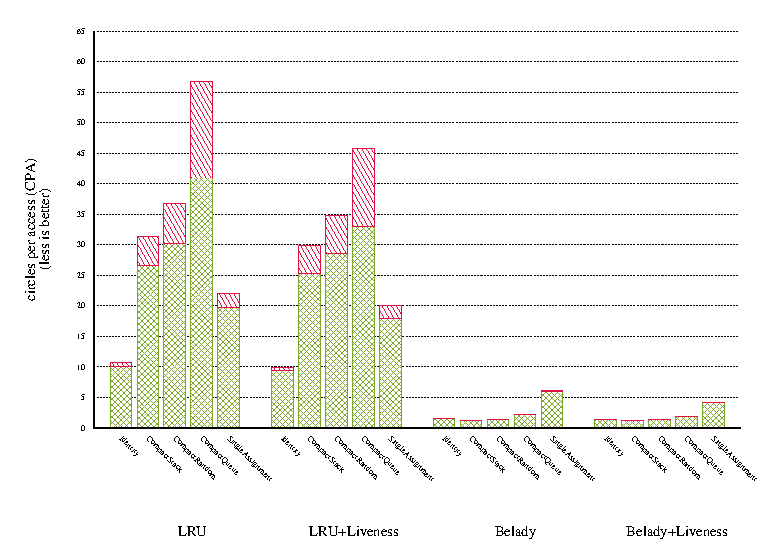
\includegraphics[width=\textwidth]{figs/plots/perf-misses-450-soplex.eps}
    \subcaption{Cache misses and cache hits}
  \end{subfigure}%
  \begin{subfigure}[b]{0.5\textwidth}%
    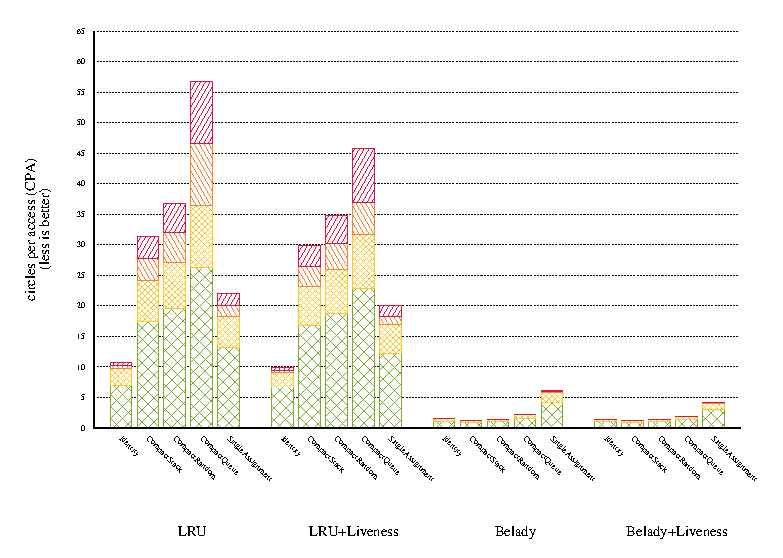
\includegraphics[width=\textwidth]{figs/plots/perf-450-soplex.eps}
    \subcaption{Types of memory operations}
  \end{subfigure}%
  \caption{Performance: 450.soplex}
  \label{fig:performance-450-soplex}
\end{figure}

\begin{figure}[!ht]
    \begin{subfigure}[b]{0.5\textwidth}%
    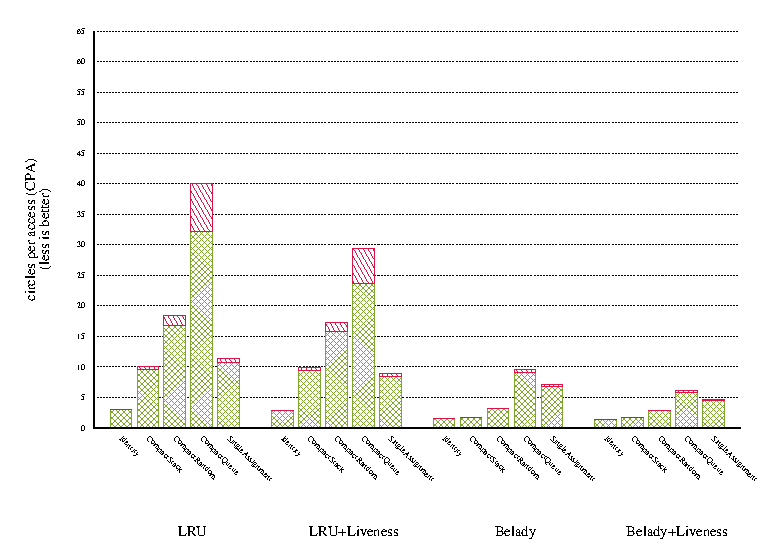
\includegraphics[width=\textwidth]{figs/plots/perf-misses-454-calculix.eps}
    \subcaption{Cache misses and cache hits}
  \end{subfigure}%
  \begin{subfigure}[b]{0.5\textwidth}%
    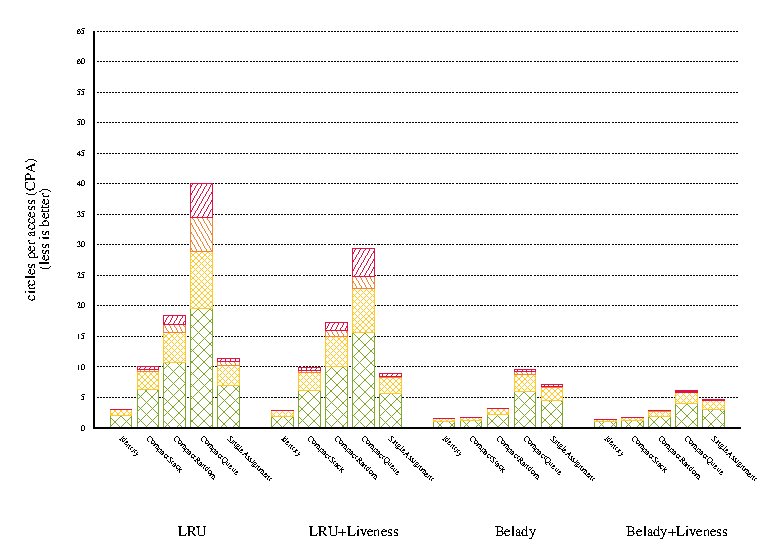
\includegraphics[width=\textwidth]{figs/plots/perf-454-calculix.eps}
    \subcaption{Types of memory operations}
  \end{subfigure}%
  \caption{Performance: 454.calculix}
  \label{fig:performance-454-calculix}
\end{figure}

\begin{figure}[!ht]
  \begin{subfigure}[b]{0.5\textwidth}%
    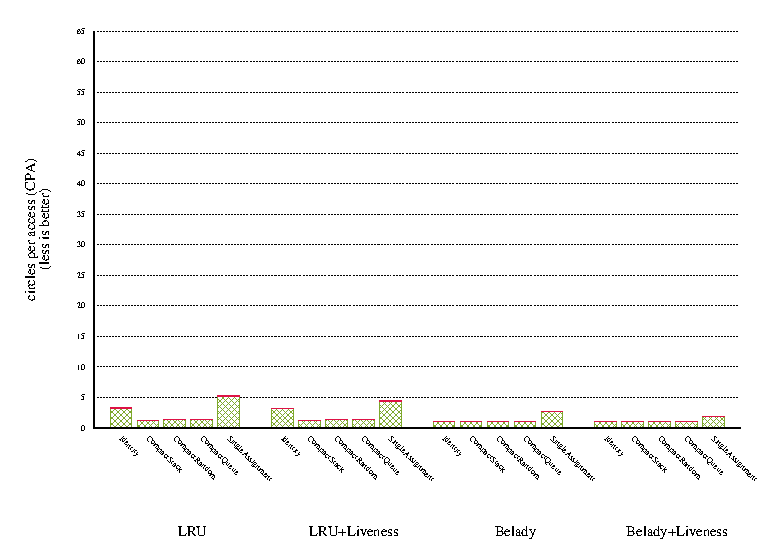
\includegraphics[width=\textwidth]{figs/plots/perf-misses-462-libquantum.eps}
    \subcaption{Cache misses and cache hits}
  \end{subfigure}%
  \begin{subfigure}[b]{0.5\textwidth}%
    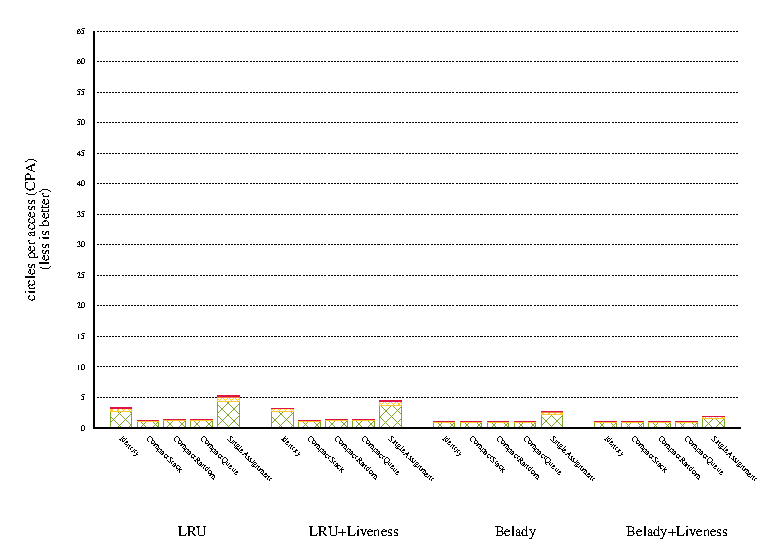
\includegraphics[width=\textwidth]{figs/plots/perf-462-libquantum.eps}
    \subcaption{Types of memory operations}
  \end{subfigure}%
  \caption{Performance: 462.libquantum}
  \label{fig:performance-462-libquantum}
\end{figure}

\begin{figure}[!ht]
  \begin{subfigure}[b]{0.5\textwidth}%
    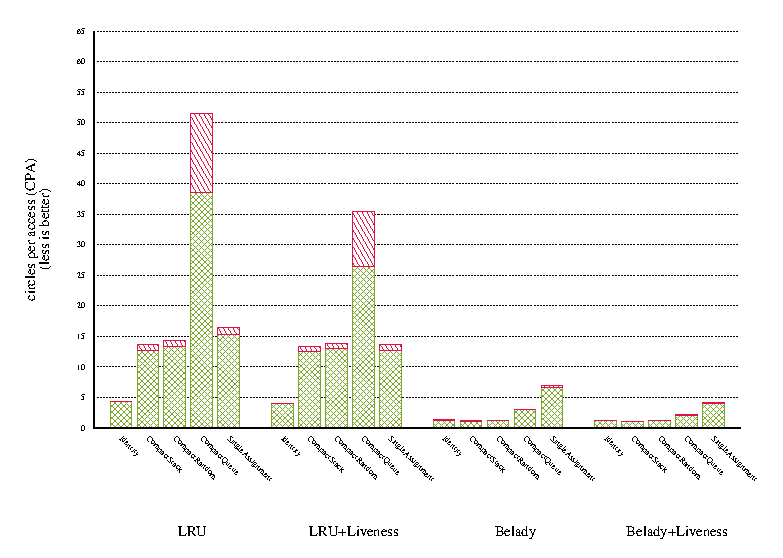
\includegraphics[width=\textwidth]{figs/plots/perf-misses-deltablue.eps}
    \subcaption{Cache misses and cache hits}
  \end{subfigure}%
  \begin{subfigure}[b]{0.5\textwidth}%
    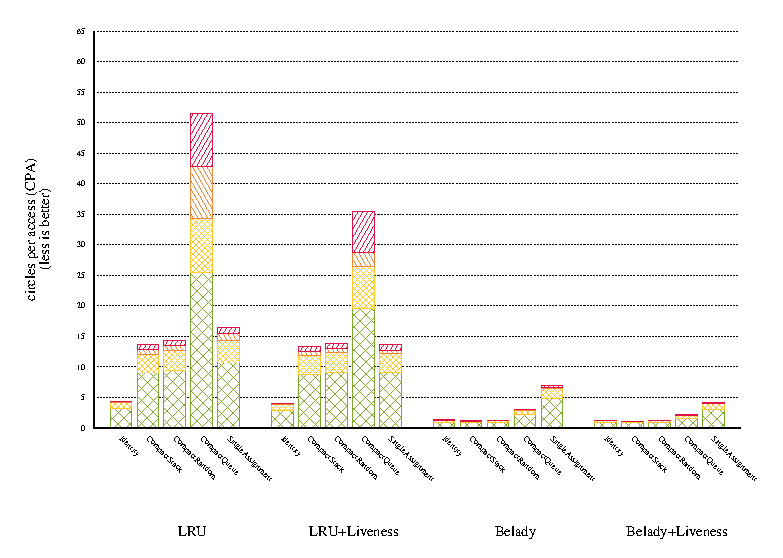
\includegraphics[width=\textwidth]{figs/plots/perf-deltablue.eps}
    \subcaption{Types of memory operations}
  \end{subfigure}%
  \caption{Performance: deltablue}
  \label{fig:performance-deltablue}
\end{figure}

\begin{figure}[!ht]
  \begin{subfigure}[b]{0.5\textwidth}%
    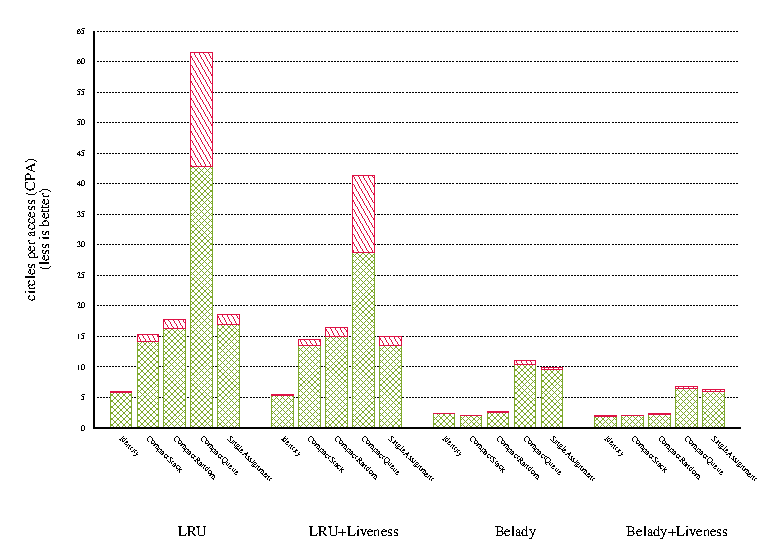
\includegraphics[width=\textwidth]{figs/plots/perf-misses-raytrace.eps}
    \subcaption{Cache misses and cache hits}
  \end{subfigure}%
  \begin{subfigure}[b]{0.5\textwidth}%
    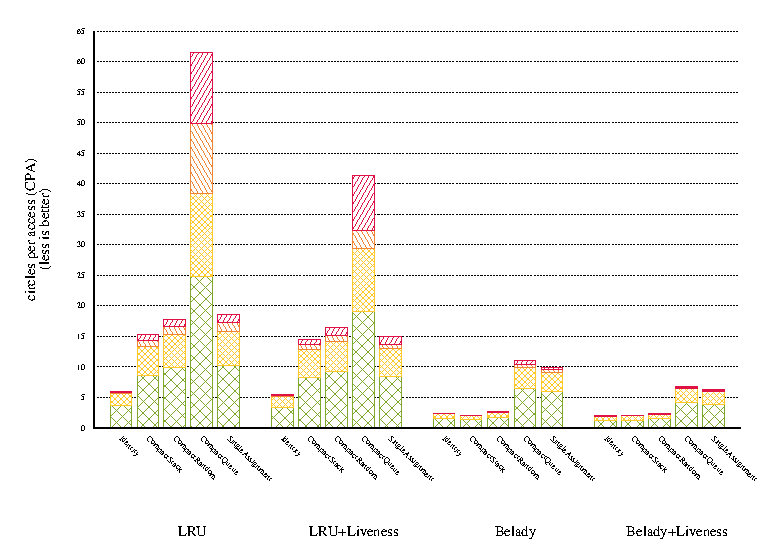
\includegraphics[width=\textwidth]{figs/plots/perf-raytrace.eps}
    \subcaption{Types of memory operations}
  \end{subfigure}%
  \caption{Performance: raytrace}
  \label{fig:performance-raytrace}
\end{figure}

\begin{figure}[!ht]
  \begin{subfigure}[b]{0.5\textwidth}%
    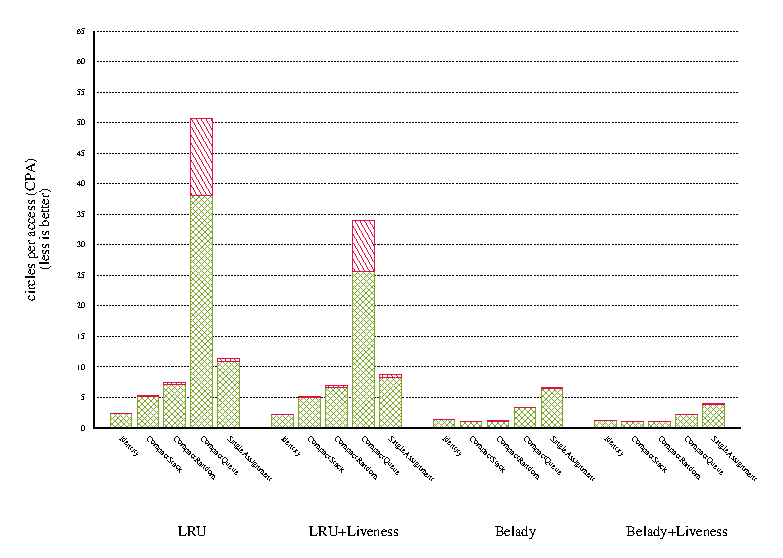
\includegraphics[width=\textwidth]{figs/plots/perf-misses-richards.eps}
    \subcaption{Cache misses and cache hits}
  \end{subfigure}%
  \begin{subfigure}[b]{0.5\textwidth}%
    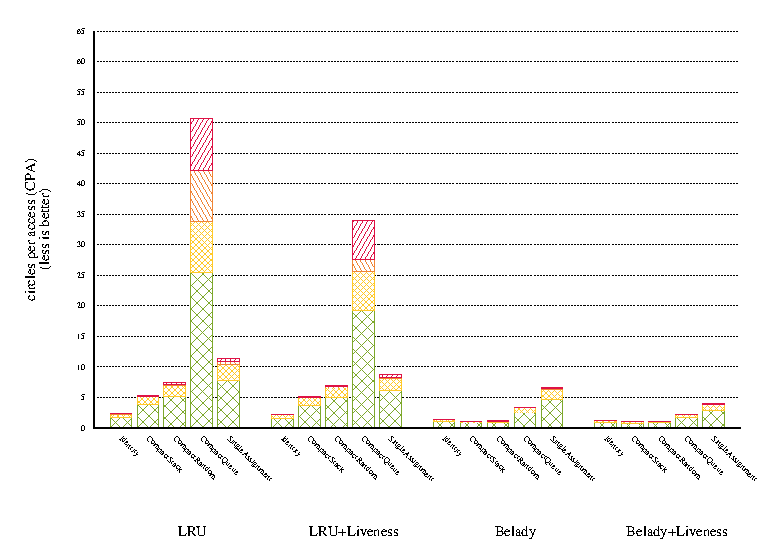
\includegraphics[width=\textwidth]{figs/plots/perf-richards.eps}
    \subcaption{Types of memory operations}
  \end{subfigure}%
  \caption{Performance: richards}
  \label{fig:performance-richards}
\end{figure}

\subsection{Speedup \& Compaction}\label{app:experiment-speedup-compaction}

\begin{figure}[!ht]
  \begin{subfigure}[b]{0.5\textwidth}%
    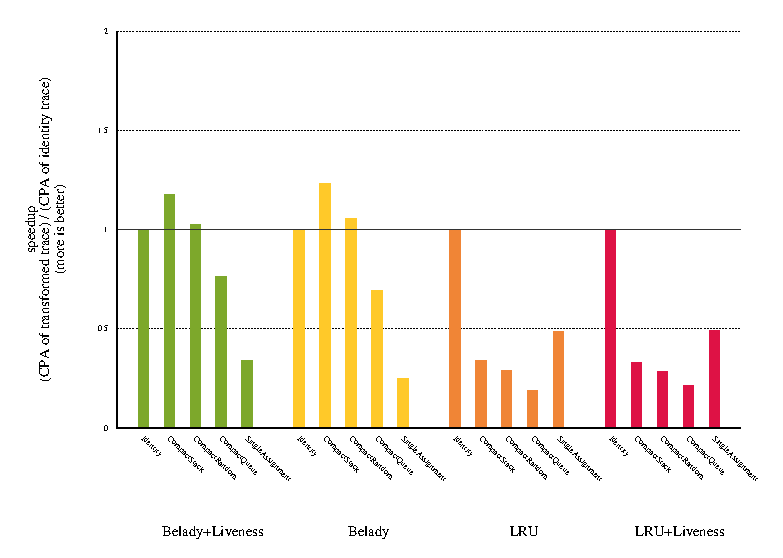
\includegraphics[width=\textwidth]{figs/plots/speedup-450-soplex.eps}
    \subcaption{Speedup}
  \end{subfigure}%
  \begin{subfigure}[b]{0.5\textwidth}%
    \includegraphics[width=\textwidth]{figs/plots/compaction-450-soplex.eps}
    \subcaption{Compaction}
  \end{subfigure}%
    \caption{Speedup \& Compaction: 450.soplex}
  \label{fig:speedup-compaction-450-soplex}
\end{figure}

\begin{figure}[!ht]
  \begin{subfigure}[b]{0.5\textwidth}%
    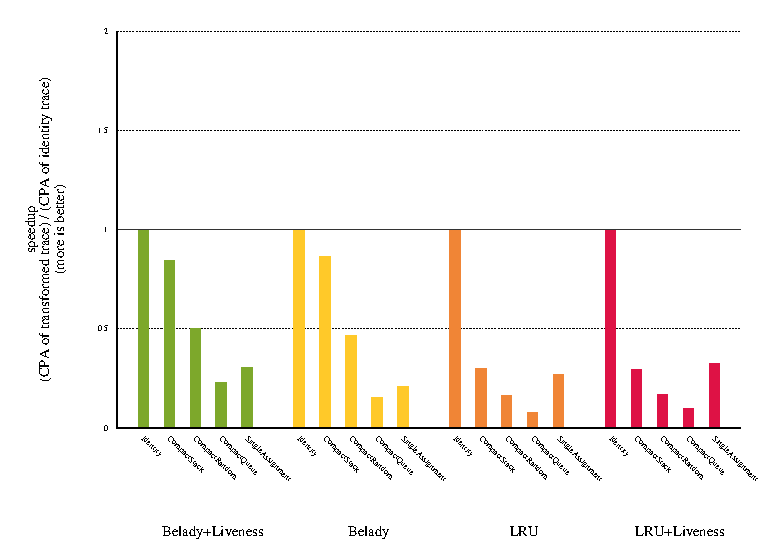
\includegraphics[width=\textwidth]{figs/plots/speedup-454-calculix.eps}
    \subcaption{Speedup}
  \end{subfigure}%
  \begin{subfigure}[b]{0.5\textwidth}%
    \includegraphics[width=\textwidth]{figs/plots/compaction-454-calculix.eps}
    \subcaption{Compaction}
  \end{subfigure}%
    \caption{Speedup \& Compaction: 454.calculix}
  \label{fig:speedup-compaction-454-calculix}
\end{figure}

\begin{figure}[!ht]
  \begin{subfigure}[b]{0.5\textwidth}%
    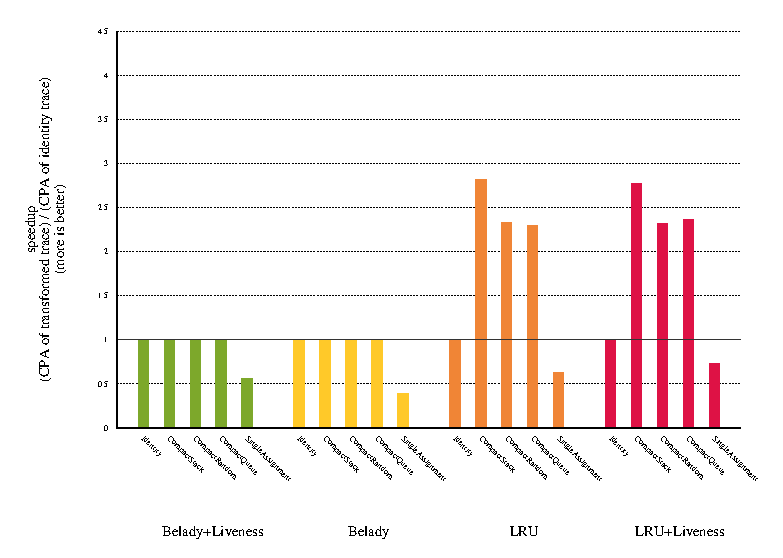
\includegraphics[width=\textwidth]{figs/plots/speedup-462-libquantum.eps}
    \subcaption{Speedup}
  \end{subfigure}%
  \begin{subfigure}[b]{0.5\textwidth}%
    \includegraphics[width=\textwidth]{figs/plots/compaction-462-libquantum.eps}
    \subcaption{Compaction}
  \end{subfigure}%
    \caption{Speedup \& Compaction: 462.libquantum}
  \label{fig:speedup-compaction-462-libquantum}
\end{figure}

\begin{figure}[!ht]
  \begin{subfigure}[b]{0.5\textwidth}%
    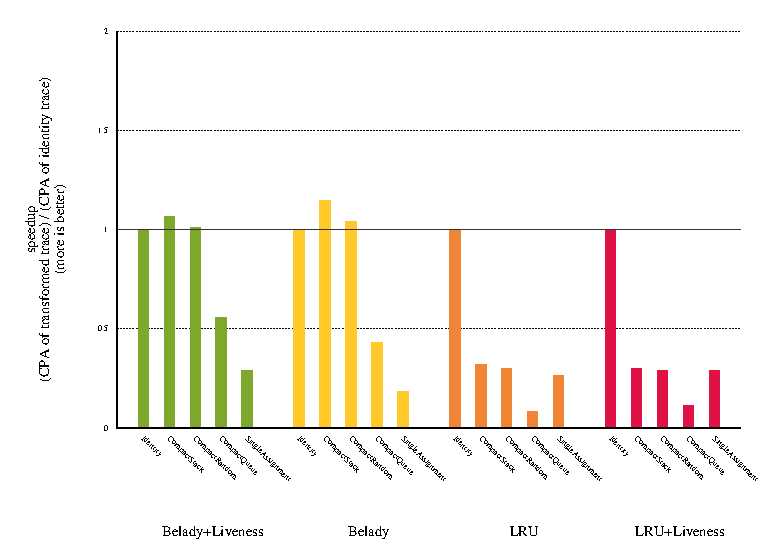
\includegraphics[width=\textwidth]{figs/plots/speedup-deltablue.eps}
    \subcaption{Speedup}
  \end{subfigure}%
  \begin{subfigure}[b]{0.5\textwidth}%
    \includegraphics[width=\textwidth]{figs/plots/compaction-deltablue.eps}
    \subcaption{Compaction}
  \end{subfigure}%
    \caption{Speedup \& Compaction: deltablue}
  \label{fig:speedup-compaction-deltablue}
\end{figure}

\begin{figure}[!ht]
  \begin{subfigure}[b]{0.5\textwidth}%
    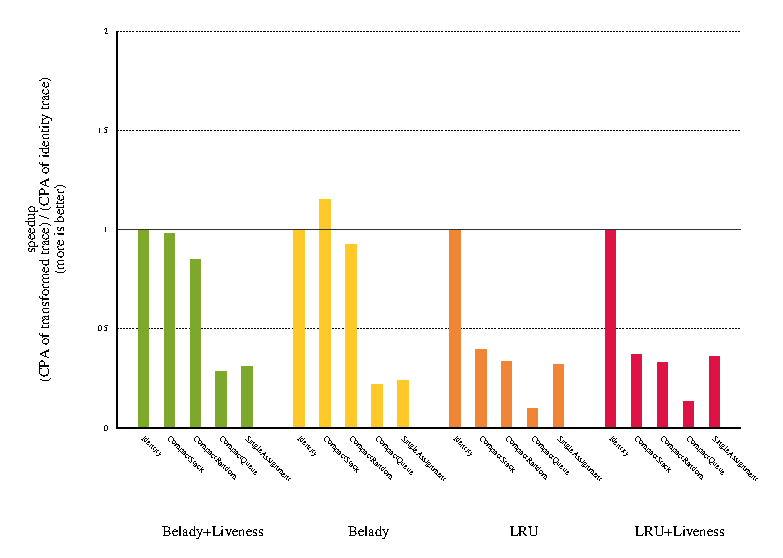
\includegraphics[width=\textwidth]{figs/plots/speedup-raytrace.eps}
    \subcaption{Speedup}
  \end{subfigure}%
  \begin{subfigure}[b]{0.5\textwidth}%
    \includegraphics[width=\textwidth]{figs/plots/compaction-raytrace.eps}
    \subcaption{Compaction}
  \end{subfigure}%
    \caption{Speedup \& Compaction: raytrace}
  \label{fig:speedup-compaction-raytrace}
\end{figure}

\begin{figure}[!ht]
  \begin{subfigure}[b]{0.5\textwidth}%
    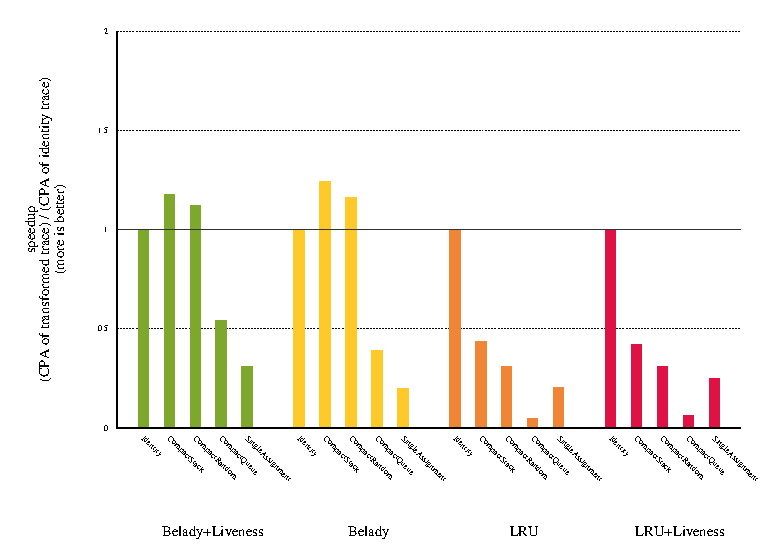
\includegraphics[width=\textwidth]{figs/plots/speedup-richards.eps}
    \subcaption{Speedup}
  \end{subfigure}%
  \begin{subfigure}[b]{0.5\textwidth}%
    \includegraphics[width=\textwidth]{figs/plots/compaction-richards.eps}
    \subcaption{Compaction}
  \end{subfigure}%
  \caption{Speedup \& Compaction: richards}
  \label{fig:speedup-compaction-richards}
\end{figure}

% \clearpage
\section{Digression on Caches}

This experimental section is distinguished into 2 parts. First we show a
few different opportunities to access a linked list, and an array,
respectively. Allows keeping our purpose in mind, we want to illustrate
the cache hierarchy. Secondly, we go into details and clarify a raising
question. Which finally leads to the answer we are looking for.

All experiments were executed on a MacBook Pro with a Intel(R) Core(TM)
i5-3230M CPU @ 2.60GHz and 3 cache levels (L1d=32KB, L1i=32KB, L2=256KB,
and L3=3MB). During the experiments there were other processes running
on the MacBook, this is why these results should be seen as proof of
concept.

\subsection{Configuration}\label{configuration-3}

The configuration is for all experiments identical.

\begin{longtable}[c]{@{}cccc@{}}
\toprule
Reps & Operations & Working Set Sizes & Addresses\tabularnewline
\midrule
\endhead
3 & 234 & 210 - 228 & 228\tabularnewline
\bottomrule
\end{longtable}

We are aware that the number of repetitions is very small, but we
consider these experiments as a \emph{proof of concept}. So 3
repetitions should be good enough.

There are parameters listed within the configuration files which are
\textbf{not} used for this experiments! These are only listed to keep
the experimental framework working.

\begin{itemize}
\tightlist
\item
  Fragmentation factor
\item
  Store ratio
\end{itemize}

As explained above we generate for each working set size a standalone
\texttt{C} file. which is complied with \texttt{gcc} in version 4.8.5
with following compiler flags \texttt{-std=c99} and \texttt{-O0}.

\hypertarget{access-opportunities}{\subsection{Access
opportunities}\label{access-opportunities}}

\hypertarget{linked-list}{\paragraph{Linked List}\label{linked-list}}

This section presents code snippets and performance results of accessing
a linked list to illustrate the cache hierarchy.

\hypertarget{sequential-access-with-2-loops}{\subparagraph{Sequential
access with 2 loops}\label{sequential-access-with-2-loops}}

The code snippet below shows how to access the linked list in a
sequential manner. All list elements are sequentially linked
corresponding to there position in (contiguous) memory. This approach
uses two nested loops.

\begin{Shaded}
\begin{Highlighting}[]
\DataTypeTok{static} \DataTypeTok{uint64_t} \NormalTok{access_read() \{}
  \KeywordTok{struct} \NormalTok{l * cur = &list[}\DecValTok{0}\NormalTok{];}
  \DataTypeTok{uint64_t} \NormalTok{start = getTimeMicrosecs();}
  \KeywordTok{for}\NormalTok{(}\DataTypeTok{int} \NormalTok{i = }\DecValTok{0}\NormalTok{; i < ITERS; i++)}
  \NormalTok{\{}
    \KeywordTok{for}\NormalTok{(}\DataTypeTok{int} \NormalTok{e = }\DecValTok{0}\NormalTok{; e < ELEMS; e++)}
    \NormalTok{\{}
      \NormalTok{cur = cur->n;}
      \NormalTok{(}\DataTypeTok{void}\NormalTok{)cur->pad[}\DecValTok{0}\NormalTok{];}
    \NormalTok{\}}
  \NormalTok{\}}
  \KeywordTok{return} \NormalTok{getTimeMicrosecs() - start;}
\NormalTok{\}}
\end{Highlighting}
\end{Shaded}

\Cref{ll-seqread-nl} presents the performance of the code above. As expected
the cache hierarchy is observable. However, performance is not that
good. How poor it really is illustrates the next experiment.

\begin{figure}[htbp]
\centering
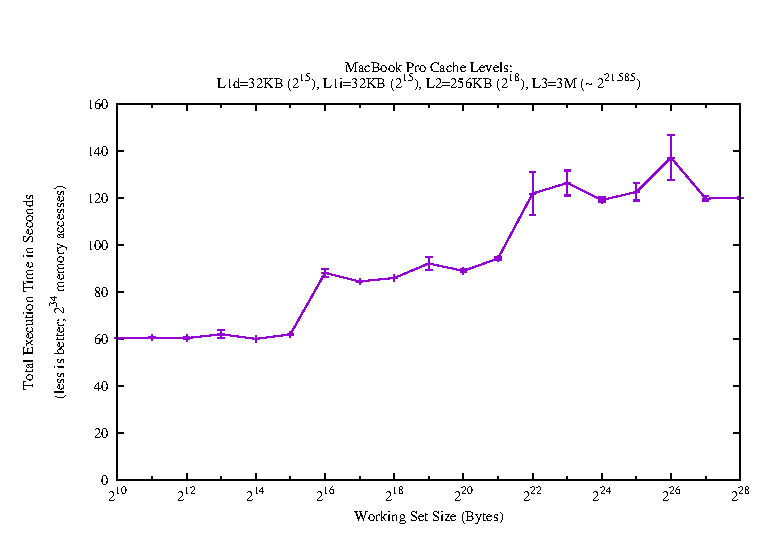
\includegraphics{appendix/plots-cache-measurements/plot-linked-list-2-loops}
\caption{Linked List, Sequential Read, and Nested Loop}
\label{ll-seqread-nl}
\end{figure}

\hypertarget{sequential-access-with-single-loop}{\subparagraph{Sequential
access with single loop}\label{sequential-access-with-single-loop}}

This approach is similar to the one above, but instead of two nested
loops a single loop is used. All list elements are sequentially linked
corresponding to there position in (contiguous) memory.

\begin{Shaded}
\begin{Highlighting}[]
\DataTypeTok{static} \DataTypeTok{uint64_t} \NormalTok{access_read() \{}
  \KeywordTok{struct} \NormalTok{l * cur = &list[}\DecValTok{0}\NormalTok{];}
  \DataTypeTok{uint64_t} \NormalTok{start = getTimeMicrosecs();}
  \KeywordTok{for}\NormalTok{(}\DataTypeTok{int} \NormalTok{i = }\DecValTok{0}\NormalTok{; i < ITERS * ELEMS; i++)}
  \NormalTok{\{}
    \NormalTok{cur = cur->n;}
    \NormalTok{(}\DataTypeTok{void}\NormalTok{)cur->pad[}\DecValTok{0}\NormalTok{];}
  \NormalTok{\}}
  \KeywordTok{return} \NormalTok{getTimeMicrosecs() - start;}
\NormalTok{\}}
\end{Highlighting}
\end{Shaded}

\Cref{app:ll-seqread-sl} illustrates the performance of the code from above. As
expected the results shows the typical shape. Remember the experiment
was not the only job running, this is why the shape not totally sharp.
This figure is used as baseline for the following experiments.

\begin{figure}[htbp]
\centering
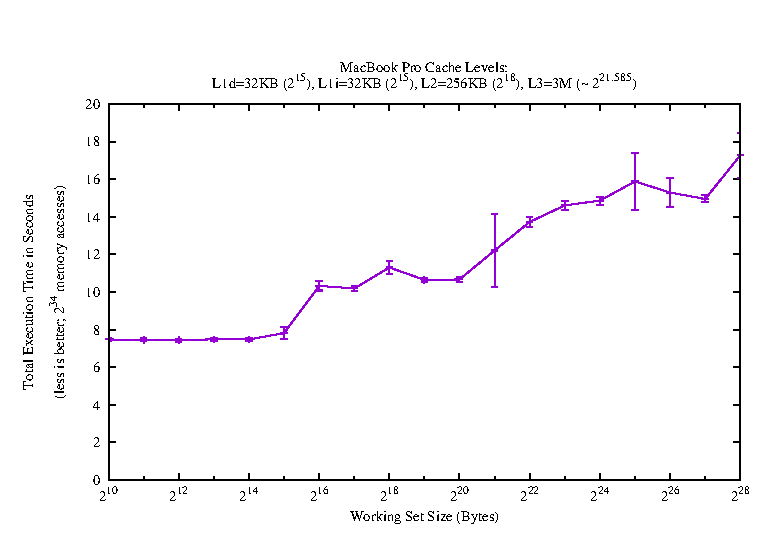
\includegraphics{appendix/plots-cache-measurements/plot-linked-list}
\caption{Linked List, Sequential Read, and Single Loop}
\label{app:ll-seqread-sl}
\end{figure}

\hypertarget{array}{\paragraph{Array}\label{array}}

This section presents different ways to compute the index of the array.
The aim is illustrate the influence of computing the index of the
current element on the actual measurements.

\hypertarget{sequential-access-with-2-loops-1}{\subparagraph{Sequential
access with 2 loops}\label{sequential-access-with-2-loops-1}}

The code snippet below shows how the array is accessed. This approach
uses to nested loop. The outer-one determines the number accesses on a
single element with the array. The inner-one ensures that keep walking
through the array.

\begin{Shaded}
\begin{Highlighting}[]
\DataTypeTok{static} \DataTypeTok{uint64_t} \NormalTok{access_read() \{}
  \DataTypeTok{uint64_t} \NormalTok{start = getTimeMicrosecs();}
  \KeywordTok{for}\NormalTok{(}\DataTypeTok{int} \NormalTok{i = }\DecValTok{0}\NormalTok{; i < ITERS; i++)}
    \KeywordTok{for}\NormalTok{(}\DataTypeTok{int} \NormalTok{j = }\DecValTok{0}\NormalTok{; j < ELEMS; j++)}
      \NormalTok{(}\DataTypeTok{void}\NormalTok{)list[j].pad[}\DecValTok{0}\NormalTok{];}
  \KeywordTok{return} \NormalTok{getTimeMicrosecs() - start;}
\NormalTok{\}}
\end{Highlighting}
\end{Shaded}

\Cref{app:arr-seqread-nl} presents the performance of the code above. Obviously
the cache hierarchy is not observable. Instead the performance seams to
be independent of the working set size. We continue with a few more
experiments on array before taking a closer look at this effect.

\begin{figure}[htbp]
\centering
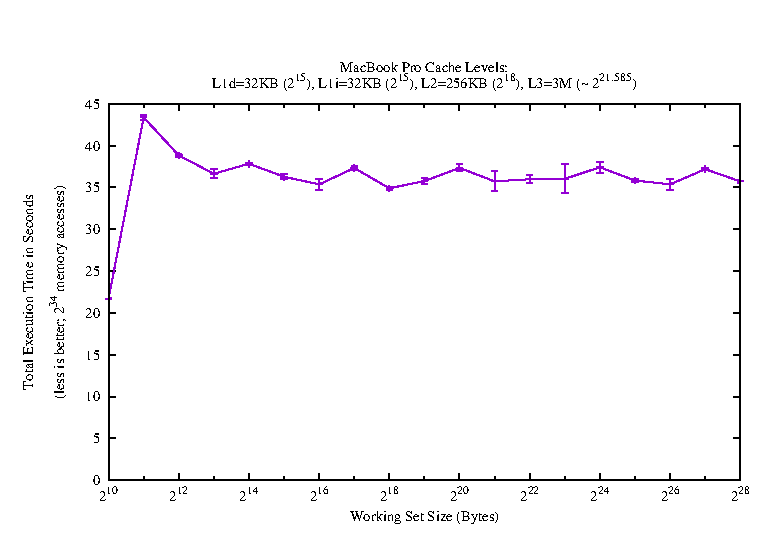
\includegraphics{appendix/plots-cache-measurements/plot-array-2-loops}
\caption{Array, Sequential Read, and Nested Loop}
\label{app:arr-seqread-nl}
\end{figure}

\hypertarget{sequential-access-with-single-loop-and-modulo}{\subparagraph{Sequential
access with single loop and
modulo}\label{sequential-access-with-single-loop-and-modulo}}

The code snippet below illustrates an approach which uses only one loop.
This requires a modulo operation to ensure to stay within the array
bounds.

\begin{Shaded}
\begin{Highlighting}[]
\DataTypeTok{static} \DataTypeTok{uint64_t} \NormalTok{access_read() \{}
  \DataTypeTok{uint64_t} \NormalTok{start = getTimeMicrosecs();}
  \KeywordTok{for}\NormalTok{(}\DataTypeTok{int} \NormalTok{i = }\DecValTok{0}\NormalTok{; i < ITERS * ELEMS; i++)}
    \NormalTok{(}\DataTypeTok{void}\NormalTok{)list[i%ELEMS].pad[}\DecValTok{0}\NormalTok{];}
  \KeywordTok{return} \NormalTok{getTimeMicrosecs() - start;}
\NormalTok{\}}
\end{Highlighting}
\end{Shaded}

\Cref{app:arr-seqread-sl} shows the performance of the code above. Again the
performance seams to be independent of the working set size. However,
there is a significant performance improvement compared to the approach
with two loops.

\begin{figure}[htbp]
\centering
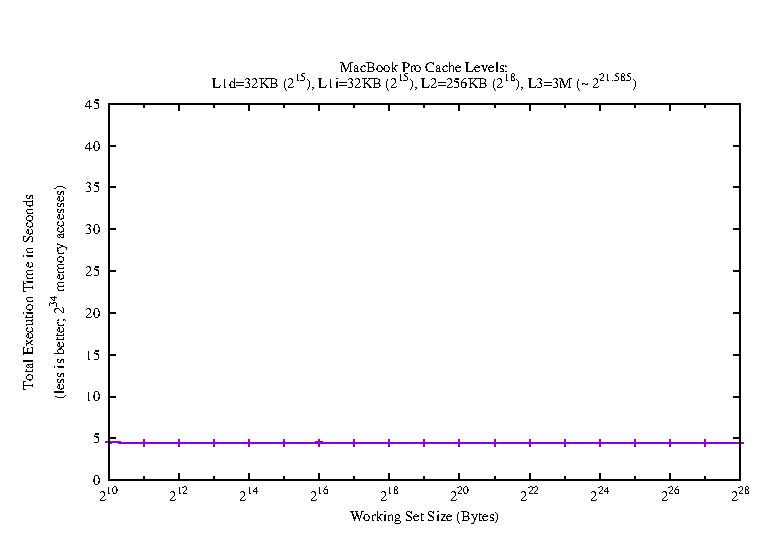
\includegraphics{appendix/plots-cache-measurements/plot-array-modulo-seq}
\caption{Array, Sequential Read, and Single Loop}
\label{app:arr-seqread-sl}
\end{figure}

\hypertarget{sequential-access-with-single-loop-and-modulo-linked-list-style}{\subparagraph{Sequential
access with single loop and modulo (linked list
style)}\label{sequential-access-with-single-loop-and-modulo-linked-list-style}}

The code snipped below presents an approach which used only one loop,
which requires a modulo operation to care about the array bounds.
Further, the coding style is like used a linked lists. There is an
additional variable \texttt{cur} which holds the address of the element
to access. The reason for this experiment that all experiments with
arrays so far do not show the cache hierarchy. To become as comparable
as possible we use this linked list like syntax.

\begin{Shaded}
\begin{Highlighting}[]
\DataTypeTok{static} \DataTypeTok{uint64_t} \NormalTok{access_read() \{}
  \KeywordTok{struct} \NormalTok{l * cur = &list[}\DecValTok{0}\NormalTok{];}
  \DataTypeTok{uint64_t} \NormalTok{start = getTimeMicrosecs();}
  \KeywordTok{for}\NormalTok{(}\DataTypeTok{int} \NormalTok{i = }\DecValTok{0}\NormalTok{; i < ITERS * ELEMS; i++)\{}
    \NormalTok{cur = &list[i%ELEMS];}
    \NormalTok{(}\DataTypeTok{void}\NormalTok{)cur->pad[}\DecValTok{0}\NormalTok{];}
  \NormalTok{\}}
  \KeywordTok{return} \NormalTok{getTimeMicrosecs() - start;}
\NormalTok{\}}
\end{Highlighting}
\end{Shaded}

\Cref{app:array-seqread-sl} below shows the performance of the code above. Again the
performance seams to be independent of the working set size. However,
the performance is slightly worse than the performance of the previous
experiment. The explanation is as simple as: It is requires to store the
address within \texttt{cur}, the approach from above computes address
and stores it in a register.

\begin{figure}[htbp]
\centering
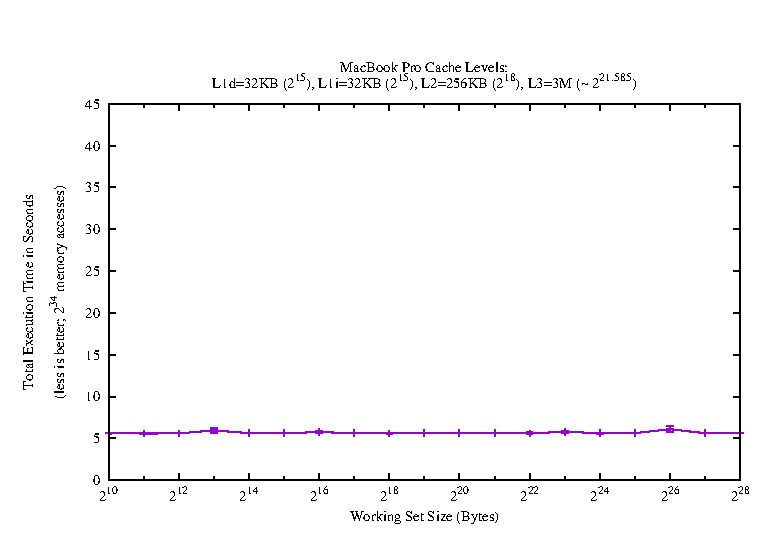
\includegraphics{appendix/plots-cache-measurements/plot-array-modulo-seq-2}
\caption{Array, Sequential Read, and Single Loop}
\label{app:array-seqread-sl}
\end{figure}

\hypertarget{sequential-access-with-single-loop-and-modulo-read-whole-payload}{\subparagraph{Sequential
access with single loop and modulo (read whole
payload)}\label{sequential-access-with-single-loop-and-modulo-read-whole-payload}}

The code snippet below presents an approach similar to those from above
with one difference: The whole payload is read (instead of simply
reading on element).

\begin{Shaded}
\begin{Highlighting}[]
\DataTypeTok{static} \DataTypeTok{uint64_t} \NormalTok{access_read() \{}
  \KeywordTok{struct} \NormalTok{l * cur = &list[}\DecValTok{0}\NormalTok{];}
  \DataTypeTok{uint64_t} \NormalTok{start = getTimeMicrosecs();}
  \KeywordTok{for}\NormalTok{(}\DataTypeTok{int} \NormalTok{i = }\DecValTok{0}\NormalTok{; i < ITERS * ELEMS; i++)\{}
    \NormalTok{cur = &list[i%ELEMS];}
    \KeywordTok{for}\NormalTok{(}\DataTypeTok{int} \NormalTok{j = }\DecValTok{0}\NormalTok{; j < NPAD; j++)}
      \NormalTok{(}\DataTypeTok{void}\NormalTok{)cur->pad[j];}
  \NormalTok{\}}
  \KeywordTok{return} \NormalTok{getTimeMicrosecs() - start;}
\NormalTok{\}}
\end{Highlighting}
\end{Shaded}

\Cref{app:array-seqreadall-sl} shows the result of the code from above. It was
expected to see the cache hierarchy, because we read the whole array
which is definitely larger than the cache. Nevertheless, the result is
the same as for the other array experiments. The only difference is the
worse performance yield by the additional loop.

\begin{figure}[htbp]
\centering
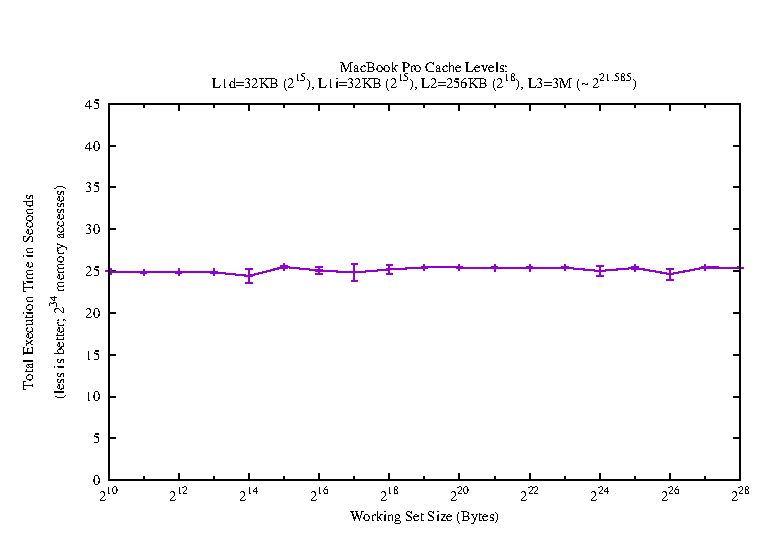
\includegraphics{appendix/plots-cache-measurements/plot-array-modulo-seq-read-all}
\caption{Array, Sequential Read All, and Single Loop}
\label{app:array-seqreadall-sl}
\end{figure}

\hypertarget{random-access-with-single-loop-and-modulo}{\subparagraph{Random
access with single loop and
modulo}\label{random-access-with-single-loop-and-modulo}}

The code snippet below presents an approach similar to those from above
with one difference: Now the array elements are access in a random
order. \texttt{mapper} contains a randomly chosen permutation of all
array indexes.

\begin{Shaded}
\begin{Highlighting}[]
\DataTypeTok{static} \DataTypeTok{uint64_t} \NormalTok{access_read() \{}
  \KeywordTok{struct} \NormalTok{l * cur = &list[}\DecValTok{0}\NormalTok{];}
  \DataTypeTok{uint64_t} \NormalTok{start = getTimeMicrosecs();}
  \KeywordTok{for}\NormalTok{(}\DataTypeTok{int} \NormalTok{i = }\DecValTok{0}\NormalTok{; i < ITERS * ELEMS; i++)\{}
    \NormalTok{cur = &list[mapper[i%ELEMS]];}
    \NormalTok{(}\DataTypeTok{void}\NormalTok{)cur->pad[}\DecValTok{0}\NormalTok{];}
  \NormalTok{\}}
  \KeywordTok{return} \NormalTok{getTimeMicrosecs() - start;}
\NormalTok{\}}
\end{Highlighting}
\end{Shaded}

The performance result is shown in \Cref{app:arr-randread-sl}. The random access order is chosen
to get rid of pre-fetching which could probably influence the execution
time. But even with random access on the array we cannot observer the
cache hierarchy. It is comparable to \emph{sequential access with single
loop and modulo (linked list style)}.

\begin{figure}[htbp]
\centering
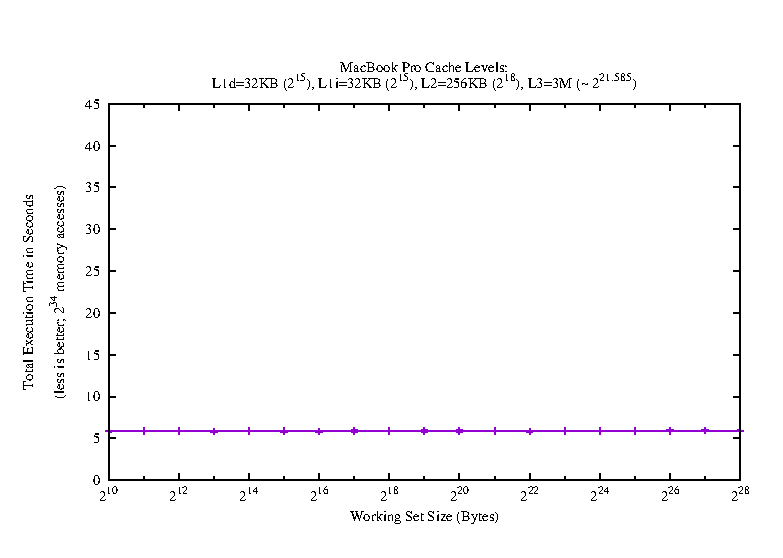
\includegraphics{appendix/plots-cache-measurements/plot-array-modulo-rand}
\caption{Array, Random Read, and Single Loop}
\label{app:arr-randread-sl}
\end{figure}

\hypertarget{summary-1}{\paragraph{Summary}\label{summary-1}}

We presented experiments on accessing two different data structures,
linked lists, and arrays, respectively. For linked lists we showed that
there is a huge performance difference in using nested loops or just a
single loop. This fact is not super surprising, but nevertheless
important to keep in mind. Also for arrays is shown that 2 nested loops
perform do not perform well. Further, we tried to measure the cache
hierarchy using just an array. Without success. Instead our experiments
show the performance differences of the different ways to access an
array. The following section will go into details why performance seams
to be independent of the working set size.

\hypertarget{the-problem}{\subsection{The problem}\label{the-problem}}

\hypertarget{definition}{\subsection{Definition}\label{definition}}

The performance curve of all experiments with array only is close to a
horizontal line, and this is unexpected behavior. It seams to be
independent of the working set size. The expected behavior would be
similar to the linked list experiments, which illustrate the cache
hierarchy.

\subsection{Analysis}\label{analysis-1}

In this section we investigate the unexpected behavior of our array
experiments from above. These experiments present constant performance
independent of the working set size.

\hypertarget{assembly-code-analysis}{\paragraph{Assembly code
analysis}\label{assembly-code-analysis}}

To simplify as much as possible we inspect only 2 code snippets from
above: - Linked list with single loop and - Array with single loop in
linked list style.

These two are the most similar one so optimal for comparison. We
disassembled the executables complied on the MacBook mentioned above.
For disassembling we are using an on-line disassembler:
\url{https://onlinedisassembler.com}.

\textbf{Linked list: C code}

\begin{Shaded}
\begin{Highlighting}[]
\DataTypeTok{static} \DataTypeTok{uint64_t} \NormalTok{access_read() \{}
  \KeywordTok{struct} \NormalTok{l * cur = &list[}\DecValTok{0}\NormalTok{];}
  \DataTypeTok{uint64_t} \NormalTok{start = getTimeMicrosecs();}
  \KeywordTok{for}\NormalTok{(}\DataTypeTok{int} \NormalTok{i = }\DecValTok{0}\NormalTok{; i < ITERS * ELEMS; i++)\{}
    \NormalTok{cur = cur->n;}
    \NormalTok{(}\DataTypeTok{void}\NormalTok{)cur->pad[}\DecValTok{0}\NormalTok{];}
  \NormalTok{\}}
  \KeywordTok{return} \NormalTok{getTimeMicrosecs() - start;}
\NormalTok{\}}
\end{Highlighting}
\end{Shaded}

\textbf{Linked list: Assembly}

\begin{verbatim}
100000ec0 <_access_read>:
100000ec0 55                     push   %rbp
100000ec1 4889e5                 mov    %rsp,         %rbp
100000ec4 4883ec20               sub    $0x20,        %rsp
100000ec8 488d0551010000         lea    0x151(%rip),  %rax # 0x100001020<_list>
100000ecf 488945f8               mov    %rax,         -0x8(%rbp)
100000ed3 e858000000             callq  0x100000f30   <_getTimeMicrosecs>
100000ed8 488945f0               mov    %rax,         -0x10(%rbp)
100000edc c745ec00000000         movl   $0x0,         -0x14(%rbp)
100000ee3 48b80000000004000000   movabs $0x400000000, %rax
100000eed 48634dec               movslq -0x14(%rbp),  %rcx
100000ef1 4839c1                 cmp    %rax,         %rcx
100000ef4 0f8319000000           jae    0x100000f13
100000efa 488b45f8               mov    -0x8(%rbp),   %rax
100000efe 488b00                 mov    (%rax),       %rax
100000f01 488945f8               mov    %rax,         -0x8(%rbp)
100000f05 8b45ec                 mov    -0x14(%rbp),  %eax
100000f08 83c001                 add    $0x1,         %eax
100000f0b 8945ec                 mov    %eax,         -0x14(%rbp)
100000f0e e9d0ffffff             jmpq   0x100000ee3
100000f13 e818000000             callq  0x100000f30   <_getTimeMicrosecs>
100000f18 482b45f0               sub    -0x10(%rbp),  %rax
100000f1c 4883c420               add    $0x20,        %rsp
100000f20 5d                     pop    %rbp
100000f21 c3                     retq   
\end{verbatim}

\textbf{Array: C code}

\begin{Shaded}
\begin{Highlighting}[]
\NormalTok{...}
\DataTypeTok{static} \DataTypeTok{uint64_t} \NormalTok{access_read() \{}
  \KeywordTok{struct} \NormalTok{l * cur = &list[}\DecValTok{0}\NormalTok{];}
  \DataTypeTok{uint64_t} \NormalTok{start = getTimeMicrosecs();}
  \KeywordTok{for}\NormalTok{(}\DataTypeTok{int} \NormalTok{i = }\DecValTok{0}\NormalTok{; i < ITERS * ELEMS; i++)\{}
    \NormalTok{cur = &list[i%ELEMS];}
    \NormalTok{(}\DataTypeTok{void}\NormalTok{)cur->pad[}\DecValTok{0}\NormalTok{];}
  \NormalTok{\}}
  \KeywordTok{return} \NormalTok{getTimeMicrosecs() - start;}
\NormalTok{\}}
\end{Highlighting}
\end{Shaded}

\textbf{Array: Assembly}

\begin{verbatim}
100000eb0 <_access_read>:
100000eb0 55                     push   %rbp
100000eb1 4889e5                 mov    %rsp,         %rbp
100000eb4 4883ec20               sub    $0x20,        %rsp
100000eb8 488d0561010000         lea    0x161(%rip),  %rax # 0x100001020<_list>
100000ebf 488945f8               mov    %rax,         -0x8(%rbp)
100000ec3 e868000000             callq  0x100000f30   <_getTimeMicrosecs>
100000ec8 488945f0               mov    %rax,         -0x10(%rbp)
100000ecc c745ec00000000         movl   $0x0,         -0x14(%rbp)
100000ed3 48b80000000004000000   movabs $0x400000000, %rax
100000edd 48634dec               movslq -0x14(%rbp),  %rcx
100000ee1 4839c1                 cmp    %rax,         %rcx
100000ee4 0f8328000000           jae    0x100000f12
100000eea 488d052f010000         lea    0x12f(%rip),  %rax # 0x100001020<_list>
100000ef1 48634dec               movslq -0x14(%rbp),  %rcx
100000ef5 4883e10f               and    $0xf,         %rcx
100000ef9 48c1e106               shl    $0x6,         %rcx
100000efd 4801c8                 add    %rcx,         %rax
100000f00 488945f8               mov    %rax,         -0x8(%rbp)
100000f04 8b45ec                 mov    -0x14(%rbp),  %eax
100000f07 83c001                 add    $0x1,         %eax
100000f0a 8945ec                 mov    %eax,         -0x14(%rbp)
100000f0d e9c1ffffff             jmpq   0x100000ed3
100000f12 e819000000             callq  0x100000f30   <_getTimeMicrosecs>
100000f17 482b45f0               sub    -0x10(%rbp),  %rax
100000f1b 4883c420               add    $0x20,        %rsp
100000f1f 5d                     pop    %rbp
100000f20 c3                     retq   
\end{verbatim}

Now we remove everything this two code snippets have in common and is
not required for our analysis. What remains should help us to understand
the difference between array and linked list. Hopefully it offers some
answers about the performance differences.

Obviously, there are only a few lines which distinguishes the code
snippets. We take only a look at the code within the loop.

The code for the linked list is quite strait. First the address of
\texttt{cur} is loaded into \texttt{rax}. Next the address of \texttt{n}
is computed. Since \texttt{n} is the first element within the
\texttt{struct} this is identical with the address of \texttt{cur}.
Finally, the address stored in \texttt{n} is moved/assigned to
\texttt{cur} itself. For reading the first element of the payload there
is no command.

The code for the array consists of a few more lines. The most important
command is the \texttt{lea} command. \texttt{lea} is a special command
available on Intel x86 architectures. This is a so called \textbf{load
effective address} instruction, designed specially of arrays. It
performs a calculation of the effective operand address, but instead of
acting on that memory location, it loads the address that would have
been accessed into a register. This and the fact that there is no
assembly instruction generated for
\texttt{(void)\ cur-\textgreater{}pad{[}0{]}} are the reasons why the
performance of arrays seams to be independent of working set size. There
is no actual memory access, the way we want it. The following
instructions do the modulo computation and finally assign the computed
address to \texttt{cur} again.

\begin{verbatim}
# linked list
<_access_read>:
loop:     ...
          jae    end_loop
          mov    -0x8(%rbp),   %rax       # load address of cur
          mov    (%rax),       %rax       # compute address of n
          mov    %rax,         -0x8(%rbp) # assignment: cur = cur->n
                                          # (void) cur->pad[0]
          ...                             # increment loop counter
          jmpq   loop
end_loop: ...

# array
<_access_read>:
loop:     ...
          jae    end_loop
          lea    0x12f(%rip),  %rax       # load list address
          movslq -0x14(%rbp),  %rcx       # load max. loop counter
          and    $0xf,         %rcx       # compute: i%ELEMS
          shl    $0x6,         %rcx       # compute: i%ELEMS
          add    %rcx,         %rax       # compute address of list element
          mov    %rax,         -0x8(%rbp) # assignment: cur = &list[i%ELEMS]
                                          # (void) cur->pad[0]
          ...                             # increment loop counter
          jmpq   loop
end_loop: ...
\end{verbatim}

\textbf{Explanations:} - Source:
\href{https://en.wikipedia.org/wiki/X86_instruction_listings}{Wikipedia}
- Variables + \texttt{-0x8(\%rbp)}: current element
(\texttt{struct\ l\ *cur}) + \texttt{-0x14(\%rbp)}: loop counter
(\texttt{int\ i}) + \texttt{0x12f(\%rip)}: the list of structs
(\texttt{struct\ list{[}ELEMS{]}}) + \texttt{\$0xf}: number of elements
(\texttt{ELEMS} = 16) + \texttt{\$0x6}: decimal number \texttt{6} -
Registers + \texttt{rax}, \texttt{rbx}, \texttt{rcx}: 64-bit register +
\texttt{rbp}: 64-bit register, holds method local variables +
\texttt{rip}: 64-bit instruction pointer register. only in the 64-bit
mode it is possible to reference data relative to the instruction
pointer, less copying of data is required. - Commands +
\texttt{movslq\ S,\ R}: Move sign-extended double word + \texttt{shl}:
Shift left + \texttt{lea}: ``Some instruction set architectures, such as
Intel x86 {[}\ldots{}{]}, have a \textbf{Load effective address}
instruction.{[}\ldots{}{]} This performs a calculation of the effective
operand address, but instead of acting on that memory location, it loads
the address that would have been accessed into a register.
{[}\ldots{}{]}'' \emph{Source:
\href{https://en.wikipedia.org/wiki/Addressing_mode\#Useful_side_effect}{Wikipedia}}

\hypertarget{further-investigations}{\paragraph{Further
investigations}\label{further-investigations}}

One issue which is identified above is that probably there are no
Assembly commands generated for the \texttt{C} code line
\texttt{(void)\ cur-\textgreater{}pad{[}0{]};}. This is not only an
issue of our array experiments. Also for the linked list experiments
these Assembly commands are missing. For simplicity reason the following
investigations are based on the linked list code. Since there are less
Assembly commands generated in total.

\hypertarget{without-accessing-pad}{\subparagraph{\texorpdfstring{Without
accessing
\texttt{pad}}{Without accessing pad}}\label{without-accessing-pad}}

This first experiment is used to confirm or refute the hypotheses that
the compiler does not generate Assembly commands for the access of
\texttt{pad}. For this purpose we remove the line
\texttt{(void)\ cur-\textgreater{}pad{[}0{]};} for the \texttt{C} code
re-compile it and again inspect it with disassembler used before
(\url{https://onlinedisassembler.com}). Both code snippets are presented
below.

\begin{Shaded}
\begin{Highlighting}[]
\DataTypeTok{static} \DataTypeTok{uint64_t} \NormalTok{access_read() \{}
  \KeywordTok{struct} \NormalTok{l * cur = &list[}\DecValTok{0}\NormalTok{];}
  \DataTypeTok{uint64_t} \NormalTok{start = getTimeMicrosecs();}
  \KeywordTok{for}\NormalTok{(}\DataTypeTok{int} \NormalTok{i = }\DecValTok{0}\NormalTok{; i < ITERS * ELEMS; i++)\{}
    \NormalTok{cur = cur->n;}
  \NormalTok{\}}
  \KeywordTok{return} \NormalTok{getTimeMicrosecs() - start;}
\NormalTok{\}}
\end{Highlighting}
\end{Shaded}

\begin{verbatim}
<_access_read>:
loop:     ...
          jae end_loop
          mov -0x8(%rbp),     %rax        # load address of cur
          mov (%rax),         %rax        # compute address of n
          mov %rax,           -0x8(%rbp)  # assignment: cur = cur->n
          ...                             # increment loop counter
          jmpq loop
end_loop: ...
\end{verbatim}

(\href{https://github.com/cksystemsgroup/SemanticLocality/blob/localizer/experiments/localizer/__meeting_20161130/assembly_tests/exp_ll_remove_cmd.txt}{complete
assembly code})

Obviously, the disassembled code is identically with the code generated
with one line more. This is why the Assembly code from above confirms
our hypotheses: There is no code generated for the \texttt{C} code
\texttt{(void)\ cur-\textgreater{}pad{[}0{]};}. Next we want to know it
the cast is the reason or line itself.

\hypertarget{remove-cast}{\subparagraph{Remove cast}\label{remove-cast}}

To find out why the compiler ignores
\texttt{(void)\ cur-\textgreater{}pad{[}0{]};} we remove the cast. This
raises a compiler warning of an unused variable.

\begin{Shaded}
\begin{Highlighting}[]
\DataTypeTok{static} \DataTypeTok{uint64_t} \NormalTok{access_read() \{}
  \KeywordTok{struct} \NormalTok{l * cur = &list[}\DecValTok{0}\NormalTok{];}
  \DataTypeTok{uint64_t} \NormalTok{start = getTimeMicrosecs();}
  \KeywordTok{for}\NormalTok{(}\DataTypeTok{int} \NormalTok{i = }\DecValTok{0}\NormalTok{; i < ITERS * ELEMS; i++)\{}
    \NormalTok{cur = cur->n;}
    \NormalTok{cur->pad[}\DecValTok{0}\NormalTok{];}
  \NormalTok{\}}
  \KeywordTok{return} \NormalTok{getTimeMicrosecs() - start;}
\NormalTok{\}}
\end{Highlighting}
\end{Shaded}

\begin{verbatim}
<_access_read>:
loop:     ...
          jae    end_loop
          mov    -0x8(%rbp),  %rax        # load address of cur
          mov    (%rax),      %rax        # compute address of n
          mov    %rax,        -0x8(%rbp)  # assignment: cur = cur->n
          ...                             # increment loop counter
          jmpq   loop
end_loop: ...
\end{verbatim}

(\href{https://github.com/cksystemsgroup/SemanticLocality/blob/localizer/experiments/localizer/__meeting_20161130/assembly_tests/exp_ll_no_cast.txt}{complete
assembly code})

This experiment shows that the casting nothing changes. The only
recognizable effect is that the compiler does not throw the warning
about a unused variable. Next we want to force the compiler to generate
code.

\hypertarget{add-assignment}{\subparagraph{Add
assignment}\label{add-assignment}}

The previous two experiments confirmed that the compiler does not
generate Assembly code for \texttt{C} code like
\texttt{(void)\ cur-\textgreater{}pad{[}0{]};}, and
\texttt{cur-\textgreater{}pad{[}0{]};}, respectively. The issues seams
to be that we do not use the data read. Even with the compiler flag
\texttt{-O0} the compiler optimizes our program a bit. Nevertheless, we
want to access this data. One way to use this data is to store it within
a variable. We give it a first try by using a method local variable.
There is one important point to think about: \textgreater{} This line
was thought to be a \textbf{read-only access}, but by the assignment it
becomes a \textbf{write access}!

\begin{Shaded}
\begin{Highlighting}[]
\DataTypeTok{static} \DataTypeTok{uint64_t} \NormalTok{access_read() \{}
  \KeywordTok{struct} \NormalTok{l * cur = &list[}\DecValTok{0}\NormalTok{];}
  \DataTypeTok{uint64_t} \NormalTok{tmp;}
  \DataTypeTok{uint64_t} \NormalTok{start = getTimeMicrosecs();}
  \KeywordTok{for}\NormalTok{(}\DataTypeTok{int} \NormalTok{i = }\DecValTok{0}\NormalTok{; i < ITERS * ELEMS; i++)\{}
    \NormalTok{cur = cur->n;}
    \NormalTok{tmp = cur->pad[}\DecValTok{0}\NormalTok{];}
  \NormalTok{\}}
  \KeywordTok{return} \NormalTok{getTimeMicrosecs() - start;}
\NormalTok{\}}
\end{Highlighting}
\end{Shaded}

\begin{verbatim}
<_access_read>:
loop:     ...
          jae    end_loop
          mov    -0x8(%rbp),  %rax        # load address of cur
          mov    (%rax),      %rax        # compute address of n
          mov    %rax,        -0x8(%rbp)  # assignment: cur = cur->n
          mov    -0x8(%rbp),  %rax        # load address of cur again
          mov    0x8(%rax),   %rax        # load pad[0] (offset 0x8)
          mov    %rax,        -0x10(%rbp) # assignment: tmp = cur->pad[0]
          ...                             # increment loop counter
          jmpq   loop
end_loop: ...
\end{verbatim}

The Assembly code from above nicely shows that
\texttt{cur-\textgreater{}pad{[}0{]}} is accessed. Furthermore, we
familiar with the pattern of loading and storing the data. As already
mentioned at the beginning of this section it is not a
\textbf{read-only} access anymore (see:
\texttt{mov\ \%rax,\ -0x10(\%rbp)}). We are now writing the data of
\texttt{cur-\textgreater{}pad{[}0{]}} into \texttt{tmp}. This is very
important to understand.

\paragraph{Summary}\label{summary-2}

The assembly code from above offers a plausible explanation of our
results from the previous section. It impressively illustrates why
linked list should be used to measure cache performance. Nevertheless,
as an open question remains is it possible to do a proper cache
measurement with arrays only?

\hypertarget{solution}{\subsection{Solution}\label{solution}}

\paragraph{Implementation}\label{implementation-4}

According to our analysis from the previous section we replace
\texttt{(void)\ cur-\textgreater{}pad{[}0{]}} by an assignment
(\texttt{tmp\ =\ cur-\textgreater{}pad{[}0{]}}). This requires a new
method local variable \texttt{tmp}.

\textbf{Linked list}

\begin{Shaded}
\begin{Highlighting}[]
\DataTypeTok{static} \DataTypeTok{uint64_t} \NormalTok{access_read() \{}
  \KeywordTok{struct} \NormalTok{l * cur = &list[}\DecValTok{0}\NormalTok{];}
  \DataTypeTok{uint64_t} \NormalTok{tmp;}
  \DataTypeTok{uint64_t} \NormalTok{start = getTimeMicrosecs();}
  \KeywordTok{for}\NormalTok{(}\DataTypeTok{int} \NormalTok{i = }\DecValTok{0}\NormalTok{; i < ITERS * ELEMS; i++)\{}
    \NormalTok{cur = cur->n;}
    \NormalTok{tmp = cur->pad[}\DecValTok{0}\NormalTok{];  }\CommentTok{// this assignment is NEW}
  \NormalTok{\}}
  \KeywordTok{return} \NormalTok{getTimeMicrosecs() - start;}
\NormalTok{\}}
\end{Highlighting}
\end{Shaded}

\begin{verbatim}
<_access_read>:
loop:     ...
          jae    end_loop
          mov    -0x8(%rbp),    %rax
          mov    (%rax),        %rax
          mov    %rax,          -0x8(%rbp)
          mov    -0x8(%rbp),    %rax
          mov    0x8(%rax),     %rax
          mov    %rax,          -0x10(%rbp)
          ...                               # increment loop counter
          jmpq   loop
end_loop: ...
\end{verbatim}

\textbf{Array}

\begin{Shaded}
\begin{Highlighting}[]
\DataTypeTok{static} \DataTypeTok{uint64_t} \NormalTok{access_read() \{}
  \KeywordTok{struct} \NormalTok{l * cur = &list[}\DecValTok{0}\NormalTok{];}
  \DataTypeTok{uint64_t} \NormalTok{tmp; }\DataTypeTok{uint64_t} \NormalTok{start = getTimeMicrosecs();}
  \KeywordTok{for}\NormalTok{(}\DataTypeTok{int} \NormalTok{i = }\DecValTok{0}\NormalTok{; i < ITERS * ELEMS; i++)\{}
    \NormalTok{cur = &list[i%ELEMS];}
    \NormalTok{tmp = cur->pad[}\DecValTok{0}\NormalTok{];  }\CommentTok{// this assignment is NEW}
  \NormalTok{\}}
  \KeywordTok{return} \NormalTok{getTimeMicrosecs() - start;}
\NormalTok{\}}
\end{Highlighting}
\end{Shaded}

\begin{verbatim}
<_access_read>:
loop:     ...
          jae    end_loop
          lea    0x12f(%rip),   %rax        # load list address
          movslq -0x1c(%rbp),   %rcx        # load max. loop counter
          and    $0xf,          %rcx        # compute: i%ELEMS
          shl    $0x6,          %rcx        # compute: i%ELEMS
          add    %rcx,          %rax        # compute address of list element
          mov    %rax,          -0x8(%rbp)  # assignment: cur = &list[i%ELEMS]
          mov    -0x8(%rbp),    %rax        # load cur address
          mov    (%rax),        %rax        # compute address of pad[0]
          mov    %rax,          -0x10(%rbp) # assignment: tmp = cur->pad[0]
          ...                               # increment loop counter
          jmpq   loop
end_loop: ...
\end{verbatim}

\paragraph{Results}\label{results-13}

\hypertarget{macbook}{\subparagraph{MacBook}\label{macbook}}

\Cref{app:correct-ll-seqacc-sl,app:correct-arr-seqacc-sl,app:correct-arr-seqaccall-sl} present the results for the two code snippets above.
Obviously, our changes had a positive effect on our measurements
especially for arrays. Instead of a nearly horizontal line we are now
able to measure the cache hierarchy also with arrays only. Comparing the
result of linked lists with the one of arrays shows that these are very
similar. This is how it should be.

\begin{figure}[htbp]
\centering
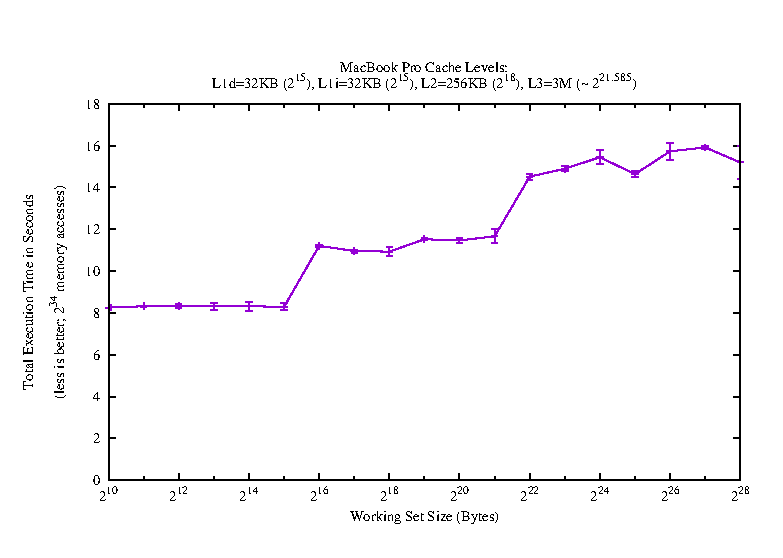
\includegraphics{appendix/plots-cache-measurements/plot-correct-ll}
\caption{Correct: Linked List, Sequential Access, and Single Loop}
\label{app:correct-ll-seqacc-sl}
\end{figure}

\begin{figure}[htbp]
\centering
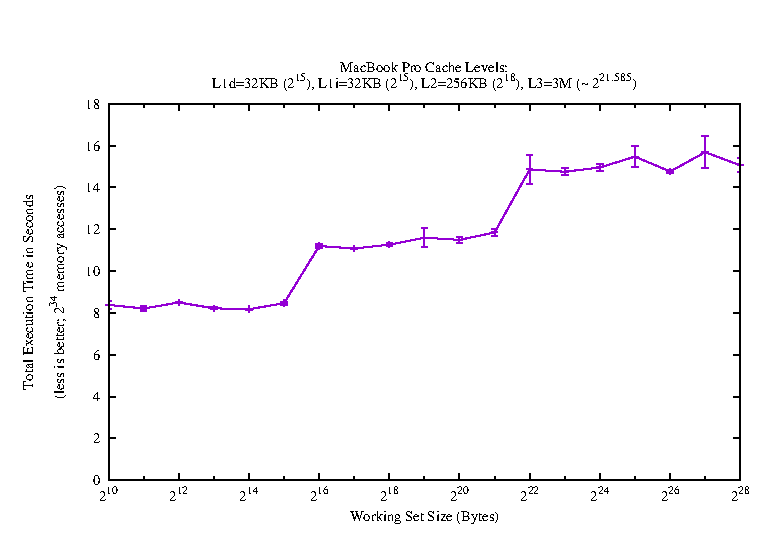
\includegraphics{appendix/plots-cache-measurements/plot-correct-array}
\caption{Correct: Array, Sequential Access, and Single Loop}
\label{app:correct-arr-seqacc-sl}
\end{figure}

\begin{figure}[htbp]
\centering
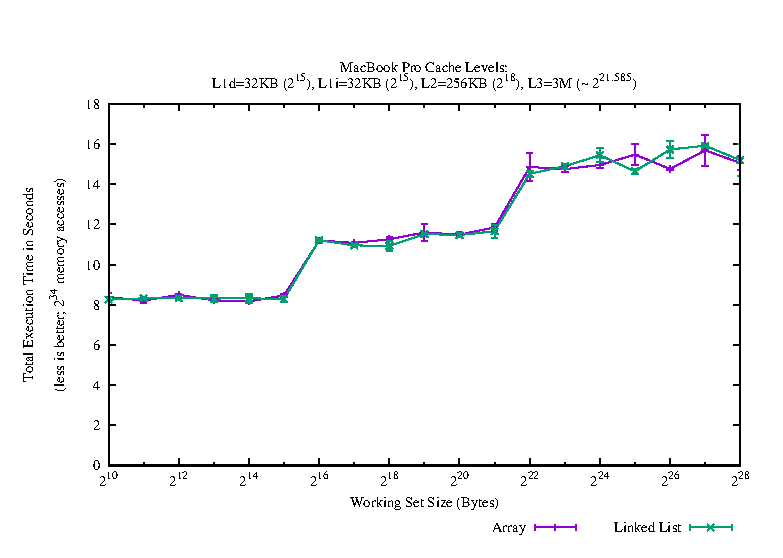
\includegraphics{appendix/plots-cache-measurements/plot-correct-array-ll}
\caption{Correct: Array, Sequential Access All, and Single Loop}
\label{app:correct-arr-seqaccall-sl}
\end{figure}

\hypertarget{big-iron9}{\subparagraph{\texorpdfstring{\texttt{big-iron9}}{big-iron9}}\label{big-iron9}}

So far all experiments are done on a MacBook pro. We re-run our approach
to solve the problem on \texttt{big-iron9} to corroborate our results.

The figure on the left shows the performance using a linked list. As
expected it illustrates nicely the cache hierarchy. We observe a
significant performance decrease at a working set size of 214 which
indicates at we now working on L2. There is another decrease around 220
which shows that L2 is not enough anymore and our data is stored in L3.
Take a look at a working set size of 224 presents the last decease of
performance, now our data is stored at the main memory.

The figure on the right shows the performance using an array. Obviously,
this approach offers better performance. This is different from the
execution on the MacBook, where performance for both approaches is quite
similar. Nevertheless, the shape of this figure presents the cache
hierarchy. We are able to observe which cache level is accessed for
which working set size. Even if the difference between L1 and L2 is very
small.

The third figure illustrates the differences of array and linked list.

\begin{figure}[htbp]
\centering
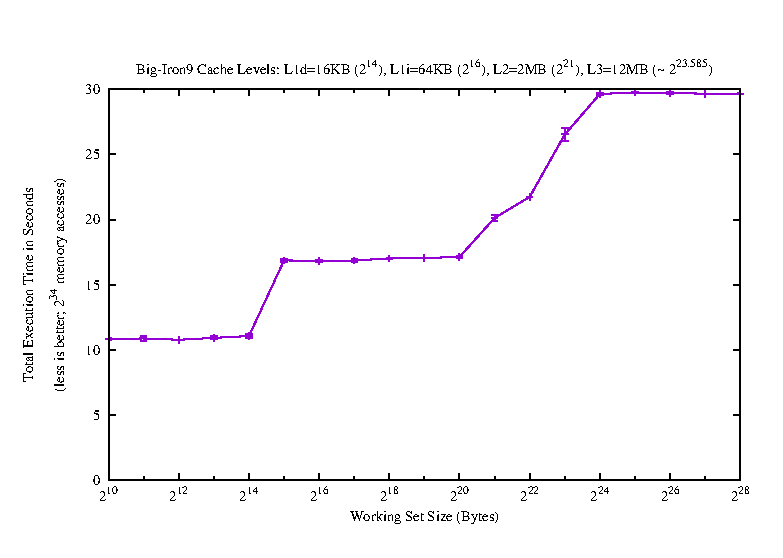
\includegraphics{appendix/plots-cache-measurements/plot-bi9-correct-ll}
\caption{Correct: Linked List, Sequential Access, and Single Loop}
\label{app:correct-ll-seqacc-sl-bi9}
\end{figure}

\begin{figure}[htbp]
\centering
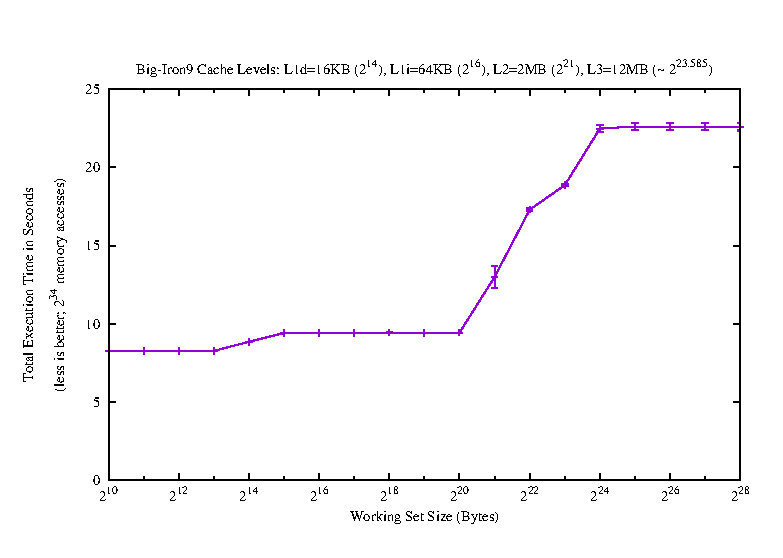
\includegraphics{appendix/plots-cache-measurements/plot-bi9-correct-array}
\caption{Correct: Array, Sequential Access, and Single Loop}
\label{app:correct-arr-seqacc-sl-bi9}
\end{figure}

\begin{figure}[htbp]
\centering
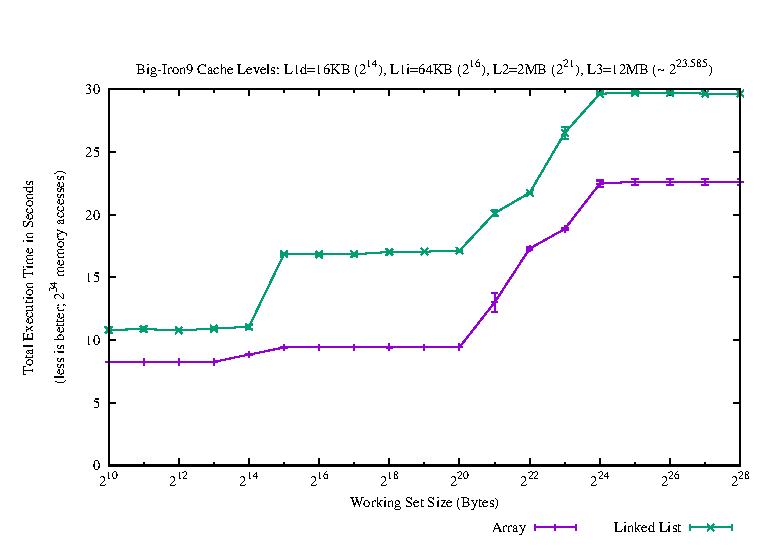
\includegraphics{appendix/plots-cache-measurements/plot-bi9-correct-array-ll}
\caption{Correct: Array, Sequential Access All, and Single Loop}
\label{app:correct-arr-seqaccall-sl-bi9}
\end{figure}

\subsection{Conclusion}\label{conclusion-5}

We started this report with experiments on different access methods of
our data structures linked list, and array, respectively. These
experiments nicely present performance differences. Furthermore, we
observe some interesting behavior for the array experiments. We define
this unexpected behavior as a problem and investigate it to find the
cause. Our investigations lead deeply into the generated assembly code.
We identified two reasons: (1) There is a special assembly command on
Intel x86 machines (\texttt{lea}) designed for array access without an
expensive memory access . (2) There are no assembly commands generated
for \texttt{C} code like \texttt{(void)cur-\textgreater{}pad{[}0{]};} if
there is no assignment. The combination of these leads to the working
set size independent performance of our array experiments. Finally, we
present a solution for this problem. Furthermore, we present experiments
which confirm the correctness of our solution.


%%%%%%%%%%%%%%%%%%%%%%%%%%%%%%%%%%%%%%%%
% List of figures/tables
\clearpage%
\listoffigures%
%
\clearpage%
\listoftables%
%
% \clearpage%
% \listofalgorithms%
%
%%%%%%%%%%%%%%%%%%%%%%%%%%%%%%%%%%%%%%%%
% Acronyms
%
\chapter{Acronyms}%
%
\begin{acronym}%
  \acro{CPA}{cycles per access}
  \acro{CPU}{central processing unit}
  \acro{LRU}{least recently used}
  \acro{trace}{memory access trace}
  \acro{MIN}{\Citeauthor{belady1966study}s algorithm}
\end{acronym}%
%
%%%%%%%%%%%%%%%%%%%%%%%%%%%%%%%%%%%%%%%
% Bibliography
%
\bibliographystyle{plainnat}%
\bibliography{references}%
%

\todo{dummy cite to activate bib: \cite{jacob2010memory}}

\end{document}



















\chapter{Introduction}
\section{Definitions - V1}
\subsection{General definitions}
\begin{definition}[Command]
A command is an instruction with the purpose to perform some specific action, e.g, to add two numbers.
\end{definition}

\begin{definition}[Data]
Data is the information required by a program for its execution, e.g., values for computations.
\end{definition}

\begin{definition}[Program]
A program consists of a sequence of commands which operate on the programs data.
\end{definition}

\begin{definition}[CPU]
The CPU (central processing unit) executes a program, i.e., command by command is processed.
\end{definition}

\begin{definition}[Main Memory (in short: memory)]
Main Memory is a physical storage. It is structured in chunks of same size. During execution of a program the main memory stores the programs data and the program itself.
\end{definition}

\begin{definition}[Address]
A physical address is an unique identifier of a single memory chunk.
\end{definition}

%  chunk             address
%  M +-------------+ m
%    &     ...     |
%    &     ...     |
%    &     ...     |
%  J +-------------+ j
%    &    Data     |
%    + - - - - - - +
%    &   Program   |
%  I +-------------+ i
%    &     ...     |
%    &     ...     |
%    &     ...     |
%  0 +-------------+ 0

\begin{definition}[Allocator]
An allocator maintains a specific part of a programs data, the so-called \textit{heap}. The purpose of an allocator is to keep track about the addresses which are currently in use by the program (\textit{allocated}) and which are not (\textit{free}).
\end{definition}

%  M +-------------+     /  J +-------------+ address j
%    &     ...     &    /     &    Stack    |
%    &     ...     &   /      + ~ ~ ~ ~ ~ ~ + (*)
%    &     ...     &  /       & Free memory |
%  J +-------------+          + ~ ~ ~ ~ ~ ~ + (*)
%    &    Data     &          &             |
%  K + - - - - - - +          &    Heap     |
%    &   Program   &          &             |
%  I +-------------+          +-------------+
%    &     ...     &  \       &  Constants  |
%    &     ...     &   \    K + - - - - - - +
%    &     ...     &    \     &   Program   |
%  0 +-------------+     \  I +-------------+ address i
%  (*) Dynamic bound: Grows and shrinks during program execution.

\begin{definition}[Memory layout]
A memory layout describes which data is stored at which address. The memory layout is determined by the allocator.
\end{definition}

\begin{example}
Following example shows two possible memory layouts for the \texttt{data 0-10}. 
%  J +-------------+ j   /  + ~ ~ ~ ~ ~ ~ +  + ~ ~ ~ ~ ~ ~ +
%    &    Stack    &    /   &   data 00   &  &   data 10   &  address (k + 10)
%    + ~ ~ ~ ~ ~ ~ +   /    &   data 01   &  &   data 09   &  address (k + 9)
%    & Free memory &  /     &   data 02   &  &   data 08   &  address (k + 8)
%    + ~ ~ ~ ~ ~ ~ +        &   data 03   &  &   data 07   &  address (k + 7)
%    &             &        &   data 04   &  &   data 06   &  address (k + 6)
%    &    Heap     &        &   data 05   &  &   data 05   &  address (k + 5)
%    &             &        &   data 06   &  &   data 04   &  address (k + 4)
%  K +-------------+ k      &   data 07   &  &   data 03   &  address (k + 3)
%    &  Constants  &  \     &   data 08   &  &   data 02   &  address (k + 2)
%    + - - - - - - +   \    &   data 09   &  &   data 01   &  address (k + 1)
%    &   Program   &    \   &   data 10   &  &   data 00   &  address (k + 0)
%  I +-------------+ i   \  +-------------+  +-------------+
\end{example}

\begin{definition}[Register]
A register is a unit of memory directly accessed by the CPU. The CPU disposes over a limited number of register to process the commands of a program. Registers store commands, addresses of data or data.
\end{definition}

%  +---------------------+   +----------------------+ 
%  & Processor           &   & Memory               |
%  & +-----+-----------+ &   & +-----------+------+ |
%  & | CPU & Registers & <---> & Addresses & Data & |
%  & +-----+-----------+ &   & +-----------+------+ |
%  +---------------------+   +----------------------+

\begin{definition}[Data access]
A data access is a command aiming on processing data of a program. 
There are two \textit{access types}:
1. \textit{read} data: load the value stored at an address into a register
2. \textit{write} data: store the value of a register at an address

In general a data access consists of 3 components: (1) an access type, (2) an address, and (3) a register. For our purpose we don't care about the register. Hence, a data access is a tuple $(t, a)$ where $t$ is an access type and $a$ is an address (within the bounds of the program).
\end{definition}

\begin{definition}[Data access time]
The data access time is the amount of time it takes to data between a register and memory or vice versa.
\end{definition}

\begin{definition}[Trace]
The trace $T$ of a program $P$ is the sequence of data accesses $((t_0, a_0), (t_1, a_1), .. (t_{N-1}, a_{N-1}))$ of $P$, with $N > 0$ and $N =|T| \leq |P|$.
\end{definition}

\begin{definition}[Liveness interval of an address]
Assume a trace $T$ which contains an address $a$. The liveness interval of $a$ begins with the first data access on $a$ and ends with the last data access on $a$.

Assume tuple $(i,j)_a$ represents the liveness interval of an address $a$ of a trace $T$, $a \in T$ with $|T| = N$ and $0 \leq i,k \leq j,l < N$, then 
 - $(t_i, a_i) \in T$ s.t. $\not\exists k < i: (t_k, a) \wedge a_i = a$, and
 - $(t_j, a_j) \in T$ s.t. $\not\exists l > j: (t_l, a) \wedge a_j = a$.
\end{definition}

\begin{definition}[Cache]
A cache is a buffer which stores data currently used by the CPU. To be more precise if there is a data access on an address, this address and its data is temporally store within the cache.
\end{definition}

\begin{quote}
\textit{Note:} Caches where introduced, because the offer a smaller data access time than main memory does. This is beneficial for the total execution time of a program.

%  +---------------------+ +---------------------------+ +----------------------+
%  & Processor           & & Cache                     & & Memory               |
%  & +-----+-----------+ & & +----------------+------+ & & +-----------+------+ |
%  & | CPU & Registers & <-> & Some Addresses & Data & <-> & Addresses & Data & |
%  & +-----+-----------+ & & +----------------+------+ & & +-----------+------+ |
%  +---------------------+ +---------------------------+ +----------------------+
\end{quote}

\begin{definition}[Cache hit]
If the CPU processes a data access on an address which is already stored in the cache, this is called a \textit{cache hit}.
\end{definition}

\begin{definition}[Cache miss]
If the CPU processes a data access on an address which is not yet stored in the cache, this is called a \textit{cache miss}.
\end{definition}

\begin{definition}[Eviction strategy]
In case of a cache miss it is required make space for the requested address and its data. The \textit{eviction strategy} decides which address is evicted from the cache, i.e., the data of this address is written back to main memory.
\end{definition}

\subsection{Performance}
\begin{definition}[Program performance]
The performance of a program is the time (milliseconds) it take the CPU to process all commands, this is called \textit{total execution time}.
\end{definition}

\begin{definition}[Allocator performance]
The performance of an allocator is the number of cache misses yield by a programs trace.
\end{definition}

\subsection{Definitions required to transform a trace $T$ into single-assignment form}
\begin{definition}[Variable]
A variable $v$ is a unique identifier of the single-assignment form. 
\end{definition}

\begin{definition}[Assignment of a variable]
Each time an data access $(t, a)$ occurs in $T$, where $t$ is a \textit{write} access a new variable $v$ is chosen to replace $a$ for this data access and all following data accesses which are of type \textit{read}. (If address $a$ of trace $T$ is written multiple times each time an new variable is used.)
\end{definition}

\begin{definition}[Static-single-assignment form (SSA)]
A program is in single-assignment form if every variable has exactly one assignment.
\end{definition}


\section{Definitions - V2}

\subsection{The Memory Hierarchy}

% +-----+ cache store  +-------+ memory store  +-------------+
% |     |------------->|       |-------------->|             |
% | CPU |              |  SPM  |               | Main Memory |
% |     |<-------------|       |<--------------|             |
% +-----+  cache load  +-------+  memory load  +-------------+

\subsubsection{About Access Times}

Wikipedia 'Cache hierarchy'\footnote{\url{https://en.wikipedia.org/wiki/Cache\_hierarchy\#Properties}} describes several properties of caches that influence cache behaviour and access times:
\begin{itemize}
  \item Banked (separation of data and instruction caches) vs unified
  \item Inclusion vs exclusion vs non-inclusive non-exclusive: Defines whether data of lower caches is duplicated in higher caches.
  \item Write through vs write back: Defines whether data is written immediately or on eviction
  \item Write allocate vs write no-allocate: Defines whether data is fetched from memory on a write miss or not.
\end{itemize}

What every programmer should know about memory\cite{drepper2007every} has these numbers for access times:

\begin{table}
  \centering
  \begin{tabular}[c]{|l|r|r|}
    \hline
    To Where & Cycles & Factor to lower memory \tabularnewline
    \hline \hline
    Register & $\leq$  1 &     - \tabularnewline
    L1d      &       \~3 &     3 \tabularnewline
    L2       &      \~14 &  4.67 \tabularnewline
    RAM      &     \~240 & 17.14 \tabularnewline
    \hline
  \end{tabular}
  \caption{\todo{add caption}}
  \label{tab:def-access-times-1}
\end{table}

The 7zip benchmark pages\footnote{\url{http://www.7-cpu.com/cpu/Skylake.html}} has cycle time numbers for modern processors. 
For example for a Intel i7-6700 (Skylake):

\begin{table}
  \centering
  \begin{tabular}[c]{|l|r|r|}
    \hline
    To Where & Latency & Factor to lower memory \tabularnewline
    \hline \hline
    L1d &                          4 or 5 cycles &  5.0 \tabularnewline
    L2  &                              12 cycles &  2.4 \tabularnewline
    L3  &                        38 or 42 cycles &  3.5 \tabularnewline
    RAM & 42 cycles + 51 ns (= 246 cycles @4GHz) & 5.86 \tabularnewline
  \end{tabular}
  \caption{\todo{add caption}}
  \label{tab:def-access-times-2}
\end{table}

\subsection{The Model}

\begin{definition}[trace]
A trace is a sequence of instructions.
\end{definition}

\begin{definition}[instruction]
An instruction is an access to an address given by the tupel $(t, a)$ with $t$ in ${Read, Write}$ and $a$ an address in main memory.
\end{definition}

\begin{definition}[Address]
A location in the memory that one variable can occupy for a certain period of time.
\end{definition}

\begin{definition}[Variable]
A value that can change overtime. In this context, a variable is a name that represents a data used by the trace. it can change according to the trace transformations.
\end{definition}

\begin{definition}[Single assignment form (SA)]
A trace is in single assignment form if every variable has exactly one assignment. \cite{rosen1988global} \cite{alpern1988detecting}
\end{definition}


\begin{definition}[Trace transformation]
Trace transformation
\end{definition}

\begin{definition}[Initial trace]
The initial trace $T$ of a program $P$ is the sequence of 'data' accesses $((t_0, a_0), (t_1, a_1), \dots (t_{N-1}, a_{N-1}))$ of $P$, with $N > 0$ and $N = |T| \leq |P|$.
\end{definition}

\begin{definition}[Data]
A data is an information processed or stored by a computer.
\end{definition}

\begin{definition}[Variable]
A variable $v$ is a unique identifier of the single-assignment form.
\end{definition}

\begin{definition}[Assignment of a variable]
Each time an data access $(t, a)$ occurs in $T$, where $t$ is a \textit{write} access a new variable $v$ is chosen to replace $a$ for this data access and all following data accesses which are of type \textit{read}. (If address $a$ of trace $T$ is written multiple times each time an new variable is used.)
\end{definition}

\begin{definition}[Canonical Form]
A canonical form trace is the trace obtained after the single Assignment transformation.
\end{definition}

\begin{definition}[Liveness interval of a variable]
The liveness interval of a variable is the continuous period of time where the variable is occupying an addresse. (the change of the addresse occupied implies a new liveness interval / "continous" means no other variable was placed in this address during this time period).
\end{definition}

% +------------+                                     +------------+
% | Trace file |                                     | Single     |
% |            | ----------------------------------> | Assignment |
% | (.trace)   |  Single Assignment Transformation   | Trace      |
% +------------+                                     +------------+

\begin{definition}[Allocator]
An allocator maintains a specific part of a programs data, the so-called \textit{heap}. The purpose of an allocator is to keep track about the addresses which are currently in use by the program (\textit{allocated}) and which are not (\textit{free}).
\end{definition}

\begin{definition}[Allocator Trace]
Allocator Trace
\end{definition}

\begin{definition}[Memory layout]
A memory layout describes which data is stored at which address. The memory layout is determined by the allocator.
\end{definition}

\begin{definition}[Address]
A location in the memory that one variable can occupy for a certain period of time.
\end{definition}

 %  chunk             address
 % M +-------------+ m
 %   |     ...     |
 %   |     ...     |
 %   |     ...     |
 % J +-------------+ j
 %   |    Data     |
 %   + - - - - - - +
 %   |   Program   |
 % I +-------------+ i
 %   |     ...     |
 %   |     ...     |
 %   |     ...     |
 % 0 +-------------+ 0

\begin{definition}[Physical Address]
A physical address is an unique identifier of a single memory chunk.
\end{definition}

\begin{definition}[Virtual Address]
A virtual address is an unique identifier of a physical address in the context of a program, i.e., there is only one virtual address 0 within a program but multiple programs might make use of an virtual address 0.
\end{definition}

\begin{definition}[Trace allocator]
The initial trace $T$ of a program $P$ is the sequence of 'addresses' accesses $((t_0, a_0), (t_1, a_1), \dots (t_{N-1}, a_{N-1}))$ of $P$, with $N > 0$ and $N = |T| \leq |P|$.
\end{definition}

\begin{definition}[Memory layout]
A memory layout describes which data is stored at which address. The memory layout is determined by the allocator.
\end{definition}

% +------------+   +-----------+   +-----------+
% | Single     |   |           |   | Allocator |
% | Assignment | + | Allocator | = | Trace     |
% | Trace      |   |           |   |           |
% +------------+   +-----------+   +-----------+

\begin{definition}[Memory Model]
Memory Model
\end{definition}

\begin{definition}[Performance]
Performance
\end{definition}

\begin{definition}[Cache]
A cache is a buffer which stores data currently used by the CPU. To be more precise if there is a data access on an address, this address and its data is temporally store within the cache.
\end{definition}

% +---------------------+ +---------------------------+ +----------------------+
% | Processor           | | Cache                     | | Memory               |
% | +-----+-----------+ | | +----------------+------+ | | +-----------+------+ |
% | | CPU | Registers | <-> | Some Addresses | Data | <-> | Addresses | Data | |
% | +-----+-----------+ | | +----------------+------+ | | +-----------+------+ |
% +---------------------+ +---------------------------+ +----------------------+

\begin{definition}[Address Spaces]
The address space is the set of addresses in the memory that will be used by the trace.
\end{definition}

\begin{definition}[Register]
A register is a unit of memory directly accessed by the CPU. The CPU disposes over a limited number of register to process the commands of a program. Registers store commands, addresses of data or data.
\end{definition}

% +---------------------+   +----------------------+
% | Processor           |   | Memory               |
% | +-----+-----------+ |   | +-----------+------+ |
% | | CPU | Registers | <---> | Addresses | Data | |
% | +-----+-----------+ |   | +-----------+------+ |
% +---------------------+   +----------------------+

\begin{definition}[Main Memory]
Main Memory is a physical storage. It is structured in chunks of same size. During execution of a program the main memory stores the programs data and the program itself.
\end{definition}

\begin{example}
Following example shows two possible memory layouts for the `data 0-10`.
% J +-------------+ j   /  + ~ ~ ~ ~ ~ ~ +  + ~ ~ ~ ~ ~ ~ +
%   |    Stack    |    /   |   data 00   |  |   data 10   |  address (k + 10)
%   + ~ ~ ~ ~ ~ ~ +   /    |   data 01   |  |   data 09   |  address (k + 9)
%   | Free memory |  /     |   data 02   |  |   data 08   |  address (k + 8)
%   + ~ ~ ~ ~ ~ ~ +        |   data 03   |  |   data 07   |  address (k + 7)
%   |             |        |   data 04   |  |   data 06   |  address (k + 6)
%   |    Heap     |        |   data 05   |  |   data 05   |  address (k + 5)
%   |             |        |   data 06   |  |   data 04   |  address (k + 4)
% K +-------------+ k      |   data 07   |  |   data 03   |  address (k + 3)
%   |  Constants  |  \     |   data 08   |  |   data 02   |  address (k + 2)
%   + - - - - - - +   \    |   data 09   |  |   data 01   |  address (k + 1)
%   |   Program   |    \   |   data 10   |  |   data 00   |  address (k + 0)
% I +-------------+ i   \  +-------------+  +-------------+
\end{example}

\begin{definition}[CPU]
The CPU (central processing unit) executes a program, i.e., command by command is processed.
\end{definition}

\begin{definition}[Data access]
A data access is a command aiming on processing data of a program. There are two \textit{access types}:
\begin{enumerate}
  \item \textit{read} data: load the value stored at an address into a register
  \item \textit{write} data: store the value of a register at an address
\end{enumerate}
In general a data access consists of 3 components: (1) an access type, (2) an address, and (3) a register. For our purpose we don't care about the register. Hence, a data access is a tuple $(t, a)$ where $t$ is an access type and $a$ is an address (within the bounds of the program).
\end{definition}

\begin{definition}[Data access time]
The data access time is the amount of time it takes to data between a register and memory or vice versa.
\end{definition}

\begin{definition}[Cache Hit]
If the CPU processes a data access on an address which is already stored in the cache, this is called a \textit{cache hit}.
\end{definition}

\begin{definition}[Cache Miss]
If the CPU processes a data access on an address which is not yet stored in the cache, this is called a \textit{cache miss}.
\end{definition}

\begin{definition}[Eviction strategy]
In case of a cache miss it is required make space for the requested address and its data. The \textit{eviction strategy} decides which address is evicted from the cache, i.e., the data of this address is written back to main memory.
\end{definition}

\subsection{Performance}
\begin{definition}[Program performance]
The performance of a program is the time it take the CPU to process all commands, this is called \textit{total execution time}
\end{definition}

\begin{definition}[Allocator performance]
The performance of an allocator is the number of cache misses yield by a programs trace.
\end{definition}

% +-----------+   +--------+
% | Allocator |   | Memory |
% | Trace     | + | Model  | = Performance metric
% |           |   |        |
% +-----------+   +--------+

\subsection{The Allocators}

\subsubsection{SingleAssignmentAllocator}
\subsubsection{IdentityAllocator}
\subsubsection{CompactStackAllocator}
\subsubsection{CompactQueueAllocator}
\subsubsection{CompactRandomAllocator}

\subsection{The Caches}
\subsubsection{BeladyCache}
\subsubsection{OPTCache}
\subsubsection{ValgrindCache}
\subsubsection{ValgrindLivenessCache}

%%%%%%%%%%%%%%%%%%%%%%%%%%%%%%%%%%%%%%%%%%%%%%%%%%%%%%%%%%%%%%%%%%%%%%%%%%%%%%%%%%%%%%%%%%%%%%%%%%%%%%%
%%%%%%%%%%%%%%%%%%%%%%%%%%%%%%%%%%%%%%%%%%%%%%%%%%%%%%%%%%%%%%%%%%%%%%%%%%%%%%%%%%%%%%%%%%%%%%%%%%%%%%%
%%%%%%%%%%%%%%%%%%%%%%%%%%%%%%%%%%%%%%%%%%%%%%%%%%%%%%%%%%%%%%%%%%%%%%%%%%%%%%%%%%%%%%%%%%%%%%%%%%%%%%%
%%%%%%%%%%%%%%%%%%%%%%%%%%%%%%%%%%%%%%%%%%%%%%%%%%%%%%%%%%%%%%%%%%%%%%%%%%%%%%%%%%%%%%%%%%%%%%%%%%%%%%%
%%%%%%%%%%%%%%%%%%%%%%%%%%%%%%%%%%%%%%%%%%%%%%%%%%%%%%%%%%%%%%%%%%%%%%%%%%%%%%%%%%%%%%%%%%%%%%%%%%%%%%%
%%%%%%%%%%%%%%%%%%%%%%%%%%%%%%%%%%%%%%%%%%%%%%%%%%%%%%%%%%%%%%%%%%%%%%%%%%%%%%%%%%%%%%%%%%%%%%%%%%%%%%%

\chapter{Experiments}

\section{Compact Allocators}

\begin{quote}
For a given trace, can I get a better (the optimal) performance simply by changing addresses?
\end{quote}

\subsection{Previous Work}

The last reports have shown that in the context of scratchpad memory and with full knowledge about the liveness of addresses the number of memory accesses is independent of the memory layout. The number of misses, however, is influenced by it.
The plots suggest that a compacting allocator which reuses cached dead items gives a transformation that is minimal in the number of misses when using a scratchpad memory model.

\begin{quote}
Given a trace $T$, liveness information of addresses of $T$, a scratchpad memory and a scratchpad strategy based on $T$. Then, a compacting allocator that reuses cached dead items when possible gives the transformed trace $T'$ that is optimal in the number of misses.
\end{quote}

This report compares several implementations of compacting allocators.

\subsection{Methodology}

We compare the following allocators.
\begin{enumerate}
  \item \textbf{Identity} Addresses are unchanged from the original trace.
  \item \textbf{SSA} Addresses are not reused.
  \item \textbf{CompactStack} Bump pointer allocator with a free list with stack semantics. Freed addresses are appended at the end and popped from the end on allocation.
  \item \textbf{CompactQueue} Bump pointer allocator with a free list with queue semantics. Freed addresses are appended at the end and taken from the beginning on allocation.
  \item \textbf{CompactRandom} Bump pointer allocator with a free list where free addresses are chosen at random on allocation.
  \item \textbf{CompactCached} Bump pointer allocator that reuses a freed, cached address if there is one or a stack-like free list otherwise.
\end{enumerate}

The memory model is again a scratchpad memory with 8-byte lines and an increasing size.

Again, the results for the V8 benchmarks Richards, Deltablue, and Raytrace are plotted.

\subsection{Results}

\subsubsection{Richards - misses}
\begin{table}
  \centering
  \begin{tabular}[c]{|l|r|r|r|r|r|r|}
    \hline
    \textbf{SPM size in bytes} & \textbf{Identity} & \textbf{SSA} & \textbf{CompactStack} & \textbf{CompactQueue} & \textbf{CompactRandom} & \textbf{CompactCached} \tabularnewline
    \hline \hline
    1024  & 19906406 & 27186015 & 14288773 & 27185933 & 14659129 & 13501287 \tabularnewline   
    2048  & 13348365 & 21797929 &  7037009 & 21797723 &  7436173 &  6334160 \tabularnewline  
    4096  &  8502161 & 19039748 &  2529214 & 19038965 &  3015836 &  2094777 \tabularnewline  
    8192  &  5997722 & 18550483 &  1587408 & 18548641 &  2135818 &  1263075 \tabularnewline  
    16384 &  5278238 & 18315329 &  1128682 & 18305995 &  1707261 &   859009 \tabularnewline 
    32768 &  5077416 & 18178226 &   857012 & 18080705 &  1449062 &   618508 \tabularnewline 
    65536 &  4495702 & 18094113 &   677410 & 17684018 &  1262799 &   466934 \tabularnewline
    \hline
  \end{tabular}
  \caption{\todo{add caption}}
  \label{tab:experiment-compact-richards-misses}
\end{table}

\begin{figure}[ht]
  \centering
  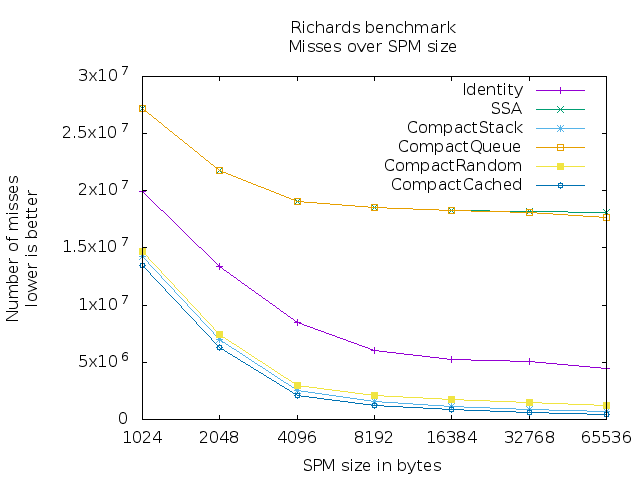
\includegraphics[width = .75\textwidth]{plots/compact-richards.png}
  \caption{Misses of Richards benchmark}
  \label{fig:experiment-compact-richards-misses}
\end{figure}

\subsubsection{DeltaBlue - misses}

\begin{table}
  \centering
  \begin{tabular}[c]{|l|r|r|r|r|r|r|}
    \hline
    \textbf{SPM size in bytes} & \textbf{Identity} & \textbf{SSA} & \textbf{CompactStack} & \textbf{CompactQueue} & \textbf{CompactRandom} & \textbf{CompactCached} \tabularnewline
    \hline \hline
    1024  & 77146231 & 98768459 & 52700195 & 98768383 & 53306777 & 50758432 \tabularnewline
    2048  & 53120872 & 79005685 & 28072125 & 79005479 & 28715840 & 25892998 \tabularnewline
    4096  & 41637998 & 70953742 & 16673778 & 70952971 & 17370985 & 14835627 \tabularnewline
    8192  & 28707195 & 65036775 &  7392572 & 65035091 &  8198850 &  6270975 \tabularnewline
    16384 & 23906668 & 62731219 &  3346997 & 62714931 &  4278582 &  2612975 \tabularnewline
    32768 & 20440744 & 62151273 &  2151620 & 62022996 &  3109816 &  1576686 \tabularnewline
    65536 & 20079036 & 61858627 &  1516174 & 61517639 &  2497068 &  1043268 \tabularnewline
    \hline
  \end{tabular}
  \caption{\todo{add caption}}
  \label{tab:experiment-compact-deltablue-misses}
\end{table}

\begin{figure}[ht]
  \centering
  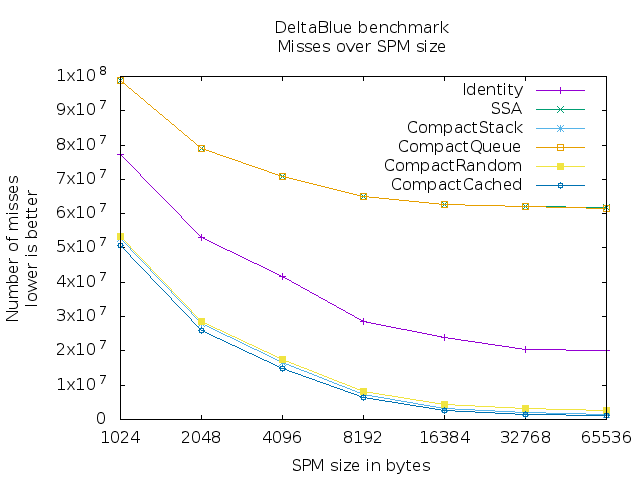
\includegraphics[width = .75\textwidth]{plots/compact-deltablue.png}
  \caption{Misses of DeltaBlue benchmark}
  \label{fig:experiment-compact-deltablue-misses}
\end{figure}

\subsubsection{Raytrace - misses}

\begin{table}
  \centering
  \begin{tabular}[c]{|l|r|r|r|r|r|r|}
    \hline
    \textbf{SPM size in bytes} & \textbf{Identity} & \textbf{SSA} & \textbf{CompactStack} & \textbf{CompactQueue} & \textbf{CompactRandom} & \textbf{CompactCached} \tabularnewline
    \hline \hline
    1024  & 17020972 & 24944756 & 11379998 & 24944674 & 11800338 & 10296539 \tabularnewline
    2048  & 14440844 & 23046938 &  8474762 & 23046732 &  8923334 &  7499105 \tabularnewline
    4096  & 12541349 & 21674551 &  6328499 & 21673768 &  6803800 &  5444919 \tabularnewline
    8192  & 10856047 & 20607354 &  4517425 & 20605669 &  5020860 &  3757431 \tabularnewline
    16384 &  9491867 & 19882091 &  3159250 & 19876330 &  3705843 &  2531928 \tabularnewline
    32768 &  8906151 & 19497833 &  2429807 & 19478760 &  2996836 &  1877661 \tabularnewline
    65536 &  8218054 & 19236973 &  1910619 & 19173814 &  2483494 &  1421185 \tabularnewline
    \hline
  \end{tabular}
  \caption{\todo{add caption}}
  \label{tab:experiment-compact-raytrace-misses}
\end{table}

\begin{figure}[ht]
  \centering
  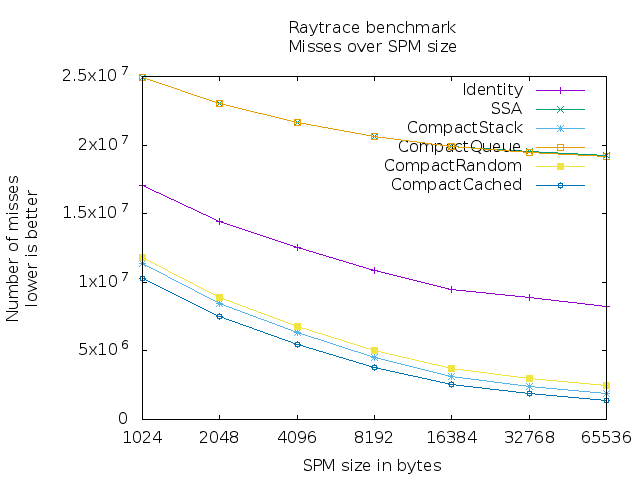
\includegraphics[width = .75\textwidth]{plots/compact-raytrace.png}
  \caption{Misses of Raytrace benchmark}
  \label{fig:experiment-compact-raytrace-misses}
\end{figure}

\subsubsection{Navier-Stokes - misses}

From Chromium Blog\footnote{\url{https://blog.chromium.org/2012/03/v8-benchmark-suite-extended-with.html}}
\begin{quote}
  This new version adds Oliver Hunt's 2D Navier-Stokes fluid dynamic simulation, which stresses intense double array computations. These complex double array computations are today common in games, graphic and scientific applications.
\end{quote}

\begin{table}
  \centering
  \begin{tabular}[c]{|l|r|r|r|r|r|r|}
    \hline
    \textbf{SPM size in bytes} & \textbf{Identity} & \textbf{SSA} & \textbf{CompactStack} & \textbf{CompactQueue} & \textbf{CompactRandom} & \textbf{CompactCached} \tabularnewline
    \hline \hline
    1024  & 151591543 & 197638846 & 122279178 & 197638770 & 124040970 & 120281818 \tabularnewline
    2048  & 126350972 & 173010778 &  96389043 & 173010573 &  98196415 &  94309498 \tabularnewline
    4096  & 123796035 & 170945407 &  93487986 & 170944635 &  95316020 &  91414571 \tabularnewline
    8192  & 121982315 & 169615053 &  91176334 & 169613376 &  93022611 &  89148010 \tabularnewline
    16384 & 118622912 & 167610304 &  87596431 & 167604544 &  89467888 &  85647336 \tabularnewline
    32768 & 114717104 & 163980384 &  81473478 & 163960984 &  83360157 &  79583462 \tabularnewline
    65536 & 106277710 & 156998071 &  70413666 & 156881332 &  72288424 &  68566643 \tabularnewline
    \hline
  \end{tabular}
  \caption{\todo{add caption}}
  \label{tab:experiment-compact-navier-stokes-misses}
\end{table}

\begin{figure}[ht]
  \centering
  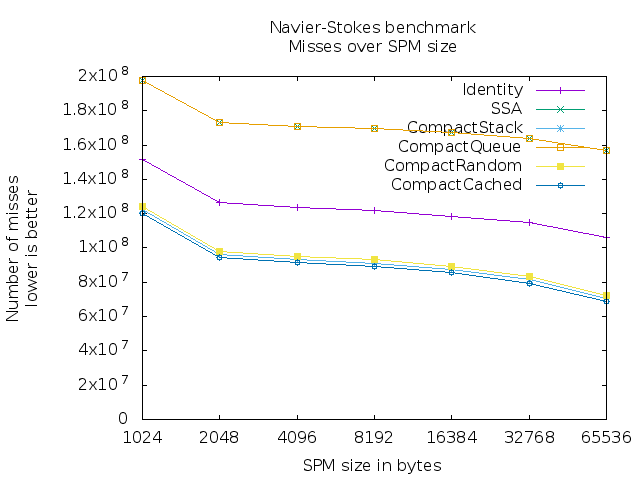
\includegraphics[width = .75\textwidth]{plots/compact-navier-stokes.png}
  \caption{Misses of Navier-Stokes benchmark}
  \label{fig:experiment-compact-navier-stokes-misses}
\end{figure}

\subsection{Conclusion}

The plots show that CompactCached has the fewest misses of all implemented compacting allocators.
Also, CompactStack has a comparable number of misses.
Interestingly also CompactRandom comes close.
We will examine if this is because of a flawed implementation or actual legit behavior.

While the plots suggest that CompactCached is better than any other examined allocator we still need solid evidence for this property.


\section{8th June, 2017 and 13th June, 2017}
\begin{quote}[Research question]
Can I get the optimal performance by changing the addresses used by a given trace $T$?
\end{quote}

\subsection{What is this report about?}
The purpose of this experiment is to show that under certain assumptions the memory layout has no impact on the number of memory accesses.

\subsection{Experimental setup}
\subsubsection{Definitions}

\begin{definition}[Instruction] 
An instruction is the pair $(t, a)$ where $t \in {R, W}$ denotes read and write access and $a$ the address being accessed.
\end{definition}

\begin{definition}[Trace] 
A trace is a sequence $((t_0, a_0), (t_1, a_1), ..., (t_{n-1}, a_{n-1}))$ of pairs with $0 \leq i < n$ where $t_i \in {R, W}$ denotes read or write access and $a_i$ the address being accessed.
\end{definition}

\begin{definition}[Liveness interval] 
A liveness interval is defined as the interval between a write to an address and the final access before the next write to the same address or the end of the trace.
\end{definition}

\begin{definition}[Trace transformation] 
We define a transformation between traces $T$ and $T'$ as a renaming of addresses such that liveness intervals are unchanged.
\end{definition}

\begin{definition}[Scratchpad memory (SPM)] 
A scratchpad memory is an application controlled, fast memory. A subset of addresses in main memory.
\end{definition}

% +-----+ store  +-------+ store  +-----+
% &     |------->|       |------->|     |
% & CPU &        &  SPM  &        & RAM |
% &     |<-------|       |<-------|     |
% +-----+  load  +-------+  load  +-----+

\begin{definition}[Memory accesses] 
A store or a load between scratchpad memory and main memory.
\end{definition}

\begin{definition}[Miss] 
Whenever the accesses item is not in the SPM it is a \textit{miss}, other wise it is a \textit{hit}.
\end{definition}

\begin{definition}[Performance] 
Performance is defined as the number of memory accesses during the the execution of a trace $T$.
\end{definition}

\begin{definition}[Optimal Performance] 
The optimal performance is the minimal number of memory accesses of all possible transformations of a trace $T$.
\end{definition}

\begin{definition}[The minimum heap size] 
Let $n_i$ $0 \leq i \leq N$ be the numbers of overlapping intervals at instruction $i$ of the trace. The minimum heap size is: $n_max * word_size$ where $n_max = \max{n_i, 0 \leq i \leq N}$.
\end{definition}

\subsection{Hypothesis}

Given a trace $T$, a scratchpad memory, liveness intervals of $T$, then the number of memory accesses is constant for any memory layout.

\subsection{Experiments}

The tiny experiment is repeated on traces of V8 benchmarks for an SPM size of $2^10$ bytes to $2^16$ bytes. Shown in this table is the number of memory accesses for each allocator as well as the average and standard deviation across all allocators.

Benchmark description taken from Chromium Blog (\url{https://blog.chromium.org/2010/10/v8-benchmark-suite-updated.html}).

\subsubsection{Tiny Example}

Take an example trace (all accesses are 8 bytes):

\begin{lstlisting}
0: W 8
1: W 16
2: W 24
3: R 16
4: R 8
5: W 32
6: R 24
7: R 32
8: R 24
9: R 16
\end{lstlisting}

We compute the misses and memory accesses of four allocators (= trace transformations):
\begin{enumerate}
\item \textbf{Identity:} Addresses are unchanged
\item \textbf{Compact:} Bump pointer allocator with a free stack
\item \textbf{Random:} Random addresses
\item \textbf{SSA:} Bump pointer without reusing of addresses
\end{enumerate}

The SPM has a size of 16 bytes and lines of 8 bytes.

Let us look at a few situations:
\begin{enumerate}
\item At instruction 2 there is a write access to address 24, the SPM contains 8 and 16. Both items in SPM are live. The item which access is the furthest in the future is chosen to be stored to main memory and replaced by the new item (see Belady's algorithm \cite{belady1966study}). This is 8 in this case. Since the new item is written to there is no need to load its content from main memory. This instruction therefore results in 1 memory access.
\item At instruction 4 there is a read request to address 8, the SPM contains 16 and 24. According to Belady 16 is selected for eviction and stored to main memory. The new item is read, therefore its content has to be loaded from main memory. This instruction results in 2 memory access.
\item At instruction 9 the address 16 is read. Both items in the SPM are dead, therefore they do not have to stored back to main memory for eviction. Regardless of the eviction choice, only the read item has to be loaded from main memory, resulting in 1 memory access for this instruction.
\end{enumerate}

The experiment is run with \texttt{semloc} and these parameters:

\begin{lstlisting}
bin/semloc -c 4 -C 4 -l 8 -L 8 -a 3 -A 3 traces/spm-example.trace 
\end{lstlisting}

The results are

\begin{table}
  \centering
  \begin{tabular}[c]{|l|c|c|}
    \hline
    \textbf{Allocator} & \textbf{Misses} & \textbf{Memory Accesses} \tabularnewline
    \hline\hline
    Identity & 6 & 4 \tabularnewline
    Compact  & 5 & 4 \tabularnewline
    Random   & 6 & 4 \tabularnewline
    SSA      & 6 & 4 \tabularnewline
    \hline
  \end{tabular}
  \caption{\todo{add caption}}
  \label{tab:experiment-2017-june-8}
\end{table}

The trace results in 4 memory access for all allocators. This suggests that memory accesses in the context of SPM are indeed independent of memory layout.

The Compact allocator has 5 misses, as opposed to all other which have 6 misses: At instruction 5 the new address 32 is written to. At this point, address 8 is dead and in the SPM. The Compact allocator reuses address 8, thus resulting in a hit. Other allocators do not exploit this possibility and have a miss at this instruction.

% \subsection{Conclusion}
% We presented the hypothesis that the memory layout does not matter for scratchpad memories, which know the trace T and liveness intervals of T. For illustrations we discussed a small example which confirms our hypothesis.

% In our example the Belady eviction policy in combination with liveness intervals make sure that memory accesses and misses remain minimal. The compact allocator only has a chance to get below that number of misses, because it turns a miss into a hit. At allocation time he can immediately achieve this by reusing a dead address in SPM.

% To conclude, this small example nicely illustrations that for systems which has certain information about there applications the memory layout has no influence.


\subsubsection{V8 benchmark: Richards}

Operating system kernel simulation benchmark originally written in BCPL by Martin Richards. The Richards benchmark effectively measures how fast the JavaScript engine is at accessing object properties, calling functions, and dealing with polymorphism. It is a standard benchmark that has been successfully used to measure the performance of many modern programming language implementations.

Trace size: 83M instructions

Memory accesses:
\begin{table}
  \centering
  \begin{tabular}[c]{|l|r|r|r|r|r|r|}
    \hline
    \textbf{SPM size in bytes} & \textbf{Identity} & \textbf{Compact} & \textbf{Random} & \textbf{SSA} & \textbf{Average} \tabularnewline
    \hline \hline
    1024  & 18654262 & 18654262 & 18654262 & 18654262 & 18654262 \tabularnewline
    2048  &  7878090 &  7878090 &  7878090 &  7878090 &  7878090 \tabularnewline
    4096  &  2361728 &  2361728 &  2361728 &  2361728 &  2361728 \tabularnewline
    8192  &  1383198 &  1383198 &  1383198 &  1383198 &  1383198 \tabularnewline
    16384 &   912890 &   912890 &   912890 &   912890 &   912890 \tabularnewline
    32768 &   638684 &   638684 &   638684 &   638684 &   638684 \tabularnewline
    65536 &   470458 &   470458 &   470458 &   470458 &   470458 \tabularnewline
    \hline
  \end{tabular}
  \caption{\todo{add caption}}
  \label{tab:experiment-2017-june-8-richards-mem}
\end{table}


Misses:
\begin{table}
  \centering
  \begin{tabular}[c]{|l|r|r|r|r|}
    \hline
    \textbf{SPM size in bytes} & \textbf{Identity} & \textbf{Compact} & \textbf{Random} & \textbf{SSA}  \tabularnewline
    \hline \hline
    1024  & 19906406 & 14288773 & 27186015 & 27186015 \tabularnewline
    2048  & 13348365 &  7037009 & 21797929 & 21797929 \tabularnewline
    4096  &  8502161 &  2529214 & 19039748 & 19039748 \tabularnewline
    8192  &  5997722 &  1587408 & 18550483 & 18550483 \tabularnewline
    16384 &  5278242 &  1128682 & 18315329 & 18315329 \tabularnewline
    32768 &  5077416 &   857012 & 18178226 & 18178226 \tabularnewline
    65536 &  4495702 &   677410 & 18094113 & 18094113 \tabularnewline
    \hline
  \end{tabular}
  \caption{\todo{add caption}}
  \label{tab:experiment-2017-june-8-richards-misses}
\end{table}

\begin{figure}[ht]
  \centering
  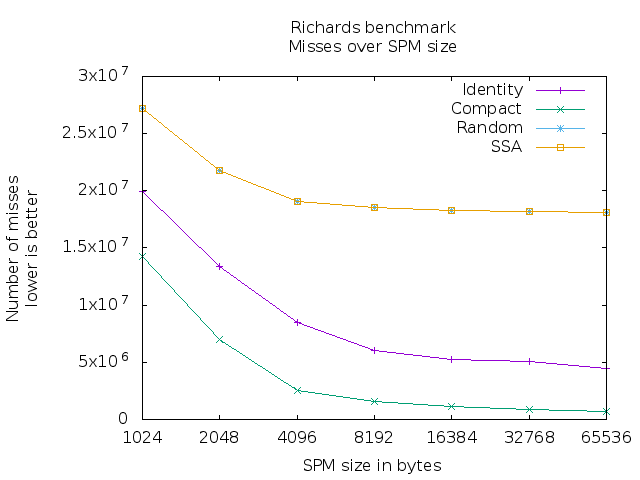
\includegraphics[width = .75\textwidth]{plots/2017-06-13-richards-misses.png}
  \caption{Misses of Richards benchmark}
  \label{fig:experiment-2017-june-8-richards-misses}
\end{figure}

\subsubsection{V8 benchmark: Deltablue}

>One-way constraint solver, originally written in Smalltalk by John Maloney and Mario Wolczko. The DeltaBlue benchmark is written in an object-oriented style with a multi-level class hierarchy. As such it measures how fast the JavaScript engine is at running well-structured applications with many objects and small functions.

Trace size: 272M instructions

Memory accesses:
\begin{table}
  \centering
  \begin{tabular}[c]{|l|r|r|r|r|r|r|}
    \hline
    \textbf{SPM size in bytes} & \textbf{Identity} & \textbf{Compact} & \textbf{Random} & \textbf{SSA} & \textbf{Average} \tabularnewline
    \hline \hline
    1024  & 74897566 & 74897566 & 74897566 & 74897566 & 74897566 \tabularnewline
    2048  & 35372018 & 35372018 & 35372018 & 35372018 & 35372018 \tabularnewline
    4096  & 19268132 & 19268132 & 19268132 & 19268132 & 19268132 \tabularnewline
    8192  &  7434198 &  7434198 &  7434198 &  7434198 &  7434198 \tabularnewline
    16384 &  2823086 &  2823086 &  2823086 &  2823086 &  2823086 \tabularnewline
    32768 &  1663194 &  1663194 &  1663194 &  1663194 &  1663194 \tabularnewline
    65536 &  1077902 &  1077902 &  1077902 &  1077902 &  1077902 \tabularnewline
    \hline
  \end{tabular}
  \caption{\todo{add caption}}
  \label{tab:experiment-2017-june-8-deltablue-mem}
\end{table}

Misses:
\begin{table}
  \centering
  \begin{tabular}[c]{|l|r|r|r|r|}
    \hline
    \textbf{SPM size in bytes} & \textbf{Identity} & \textbf{Compact} & \textbf{Random} & \textbf{SSA}  \tabularnewline
    \hline \hline
    1024  & 77146231 & 52700195 & 98768459 & 98768459 \tabularnewline
    2048  & 53120872 & 28072125 & 79005685 & 79005685 \tabularnewline
    4096  & 41637998 & 16673778 & 70953742 & 70953742 \tabularnewline
    8192  & 28707195 &  7392572 & 65036775 & 65036775 \tabularnewline
    16384 & 23906672 &  3346997 & 62731219 & 62731219 \tabularnewline
    32768 & 20440744 &  2151620 & 62151273 & 62151273 \tabularnewline
    65536 & 20079036 &  1516174 & 61858627 & 61858627 \tabularnewline
    \hline
  \end{tabular}
  \caption{\todo{add caption}}
  \label{tab:experiment-2017-june-8-deltablue-misses}
\end{table}

\begin{figure}[ht]
  \centering
  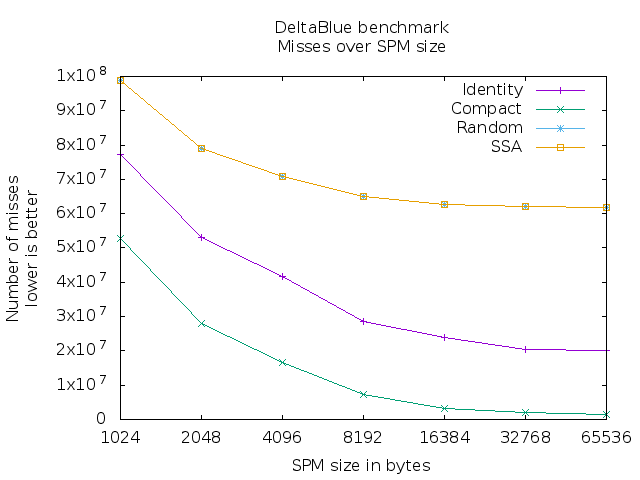
\includegraphics[width = .75\textwidth]{plots/2017-06-13-deltablue-misses.png}
  \caption{Misses of Deltablue benchmark}
  \label{fig:experiment-2017-june-8-deltablue-misses}
\end{figure}

\subsubsection{V8 benchmark: Raytrace}

Ray tracer benchmark based on code by Adam Burmister. The benchmark measures floating-point computations where the object structure is constructed using the Prototype JavaScript library.

Trace size: 62M instructions

Memory accesses:
\begin{table}
  \centering
  \begin{tabular}[c]{|l|r|r|r|r|r|r|}
    \hline
    \textbf{SPM size in bytes} & \textbf{Identity} & \textbf{Compact} & \textbf{Random} & \textbf{SSA} & \textbf{Average} \tabularnewline
    \hline \hline
    1024  & 12897373 & 12897373 & 12897373 & 12897373 & 12897373 \tabularnewline
    2048  &  9101737 &  9101737 &  9101737 &  9101737 &  9101737 \tabularnewline
    4096  &  6356963 &  6356963 &  6356963 &  6356963 &  6356963 \tabularnewline
    8192  &  4222569 &  4222569 &  4222569 &  4222569 &  4222569 \tabularnewline
    16384 &  2772043 &  2772043 &  2772043 &  2772043 &  2772043 \tabularnewline
    32768 &  2003527 &  2003527 &  2003527 &  2003527 &  2003527 \tabularnewline
    65536 &  1481807 &  1481807 &  1481807 &  1481807 &  1481807 \tabularnewline
    \hline
  \end{tabular}
  \caption{\todo{add caption}}
  \label{tab:experiment-2017-june-8-raytrace-mem}
\end{table}

Misses:
\begin{table}
  \centering
  \begin{tabular}[c]{|l|r|r|r|r|}
    \hline
    \textbf{SPM size in bytes} & \textbf{Identity} & \textbf{Compact} & \textbf{Random} & \textbf{SSA}  \tabularnewline
    \hline \hline
    1024  & 17020972 & 11379998 & 24944756 & 24944756 \tabularnewline
    2048  & 14440844 &  8474762 & 23046938 & 23046938 \tabularnewline
    4096  & 12541349 &  6328499 & 21674551 & 21674551 \tabularnewline
    8192  & 10856047 &  4517425 & 20607354 & 20607354 \tabularnewline
    16384 &  9491871 &  3159250 & 19882091 & 19882091 \tabularnewline
    32768 &  8906151 &  2429807 & 19497833 & 19497833 \tabularnewline
    65536 &  8218054 &  1910619 & 19236973 & 19236973 \tabularnewline
    \hline
  \end{tabular}
  \caption{\todo{add caption}}
  \label{tab:experiment-2017-june-8-raytrace-misses}
\end{table}

\begin{figure}[ht]
  \centering
  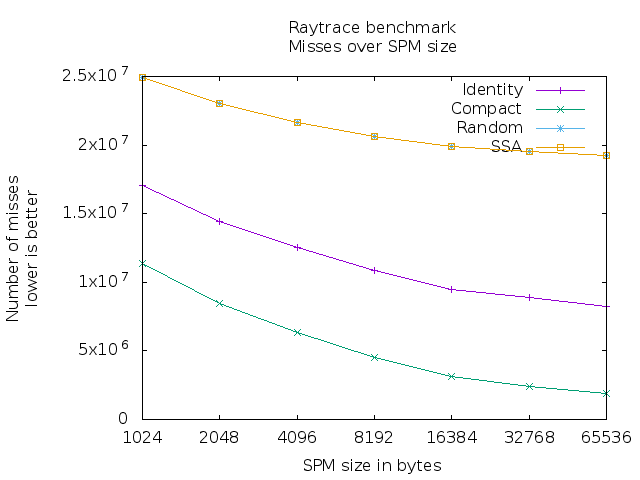
\includegraphics[width = .75\textwidth]{plots/2017-06-13-raytrace-misses.png}
  \caption{Misses of Raytrace benchmark}
  \label{fig:experiment-2017-june-8-raytrace-misses}
\end{figure}

\subsection{Conclusion}
We presented the hypothesis that the memory layout does not matter for scratchpad memories, which know the trace T and liveness intervals of T. For illustrations we discussed a small example which confirms our hypothesis.

In our example, the Belady eviction policy in combination with liveness intervals makes sure that memory accesses and misses remain minimal. The compact allocator only has a chance to get below that number of misses, because it turns a miss into a hit. At allocation time he can immediately achieve this by reusing a dead address in SPM.

To conclude, this small example nicely illustrations that for systems which have certain information about their applications the memory layout has no influence.

\subsection{Further steps}
In this (mini) report we have shown empirically that memory access is constant for all memory layouts. next, we have to prove that a compact allocator as we described in the conclusion is optimal with regards to cache misses in this SPM environment.

\section{27th July, 2017}

\subsection{Experiment: \textit{Bug fix}}
\begin{itemize}
  \item Rerun the experiments of this report, because of the counting bug fix of the LRU caches.
  \item \textit{Expectations:} The number of cycles per instruction for both LRU caches will shrink. Still we expect at both LRU implementations perform worse than OPTCache and BeladyCache.
\end{itemize}

\subsection{Experiment: \textit{Compact-Random-Allocator performance robustness}}
\begin{itemize}
  \item Find a trace optimized for the Compact-Queue-Allocator (Compact-Queue-Allocator performs better than the Compact-Stack-Allocator)
  \item Find a trace optimized for the Compact-Stack-Allocator (Compact-Stack-Allocator performs better than the Compact-Queue-Allocator)
  \item \textit{Expectations:} A good/an interesting result would be if the Compact-Random-Allocator performs (nearly) as good as the Compact-Stack-Allocator, and Compact-Queue-Allocator, respectively.
  \item \textit{Notes}
  \begin{itemize}
    \item 2017-07-31: Right now we think that it is not possible with a free list implementation based on a queue to outperform an stack implementation.
    \begin{itemize}
      \item Either the \textit{most-recently-freed} address is not in the cache anymore, then both implementations force a \textit{cache miss}.
      \item Or the \textit{most-recently-freed} address is still in the cache, then the stack implementation results in a \textit{cache hit} and the queue implementation results in a \textit{cache miss}.
    \end{itemize}
    \item Intuitively by counter-example. Assume high enough associativity. Assume CompactQueue is better than CompactStack in the same situation (same access, same state of free list), i.e. allocation  to address $a$ using CompatQueue results in a cache hit and to address $b$ with CompactStack in a cache miss. Order in free list $a < \dots < b$ and $a \not= b$. Since a free is an access this means that the last access of $a$ was before $b$. Since we have an LRU cache this would imply that $b$ was evicted before $a$, contradicting the access order.
  \end{itemize}
\end{itemize}

\subsection{Experiment: \textit{Associativity influence on LRU caches}}
\begin{itemize}
  \item Pick one of the experiments above, namely Richards.
  \item Pick one fixed cache size 
  \begin{itemize}
    \item either 1024 bytes (very small -> a lot of loads/stores)
    \item or 32KB (more realistic: l1d size of big-iron8 and MacBook Pro)
  \end{itemize}
  \item Run this experiment for different associativities of the LRU caches, e.g, 4, 8, 16, 32, fully
  \item \textit{Expectations:} The number of cycles per instruction should be identical for all associativities of the LRU caches to show that these are independent of the associativity.
\end{itemize}

\subsection{Experiment: \textit{Equally weight stores and loads (cache)}}
\begin{itemize}
  \item Generate some of the performance-indexed-figures with different weight for load and store operations.
  \item Pick two fixed cache sizes, namely 1KB and 64KB.
  \item Pick all 4 experiments from above.
  \item Pick the store-weights as multiples of the load-weights (based on the cache-loads, and cache-stores figures), e.g, 2, 3, 5, 10, ...
  \item \textit{Expectations:} The influence of the store-weight should become recognizable for unrealistic are values. To conclude it is reasonable to weight loads and stores the same.
\end{itemize}

\subsection{Experiment: \textit{Equally weight stores and loads (memory)}}
\begin{itemize}
  \item Same as for the cache loads and stores.
\end{itemize}

\subsection{Experiment: \textit{New benchmarks}}
\begin{itemize}
  \item Find new benchmarks apart of the V8 benchmarks (Richards, Raytrace, Deltablue, and Navier-stroke).
  \item Based on the Scalloc paper try to get access to the SPEC CPU2006 benchmarks.
  \begin{itemize}
    \item Generate traces.
    \item Rerun SemanticLocality with the new traces.
    \item Generate performance-indexed-figures.
  \end{itemize}
  \item \textit{Expectations:} Either confirmation of your previous results or new deep knowledge of the behavior of the caches and allocators, respectively.
\end{itemize}

\section{4th August, 2017}
\subsection{Bubble Pie Chart}

Colors
\begin{itemize}
  \item Hits in green, misses in red
  \item Cache loads, cache store, memory store, memory loads in green, yellow, orange, and red
  \item "Less is better" instead of "Lower is better"
  \item Relative and absolute number of trace reads and writes (= cache stores and loads) in legend of the plot
\end{itemize}

\subsection{Associativity Experiment}
Absolute numbers are enough

\subsection{Line Size}
\begin{itemize}
  \item Try 2 words
  \item A compacting allocator with a \textit{spatial locality threshold} $c$: The allocator remembers the last original address $a$. If a new address for $a+n$ is requested with $n \leq c$, then the allocator looks at the top 2 elements in the free stack and returns the one that is on the same cache line as the address for $a$, or any of the two if there is none.
  \item Change Belady for multi-word lines (next access data structure)
  \item Line size as CLI argument (no range, just a single value)
\end{itemize}

\subsection{Bar chart for number of addresses for all allocators}
Number of different addresses is print as a new column in the experiment results

\subsection{Workload for poor performance of CompactRandom}
\todo{no signs of interests in this direction by Christoph}

\subsection{Description why CompactQueue can never be better than CompactStack}
Intuitively by counter-example. Assume high enough associativity. Assume CompactQueue is better than CompactStack in the same situation (same access, same state of free list), i.e. allocation  to address $a$ using CompatQueue results in a cache hit and to address b with CompactStack in a cache miss. Order in free list $a < \dots < b$ and $a \not= b$. Since $a$ free is an access this means that the last access of $a$ was before $b$. Since we have an LRU cache this would imply that $b$ was evicted before $a$, contradicting the access order.

\todo{copy paste old content}